%%% The main file. It contains definitions of basic parameters and includes all other parts.

%% Settings for single-side (simplex) printing
% Margins: left 40mm, right 25mm, top and bottom 25mm
% (but beware, LaTeX adds 1in implicitly)
\documentclass[12pt,a4paper]{report}
\setlength\textwidth{145mm}
\setlength\textheight{247mm}
\setlength\oddsidemargin{15mm}
\setlength\evensidemargin{15mm}
\setlength\topmargin{0mm}
\setlength\headsep{0mm}
\setlength\headheight{0mm}
% \openright makes the following text appear on a right-hand page
\let\openright=\clearpage

%% Settings for two-sided (duplex) printing
% \documentclass[12pt,a4paper,twoside,openright]{report}
% \setlength\textwidth{145mm}
% \setlength\textheight{247mm}
% \setlength\oddsidemargin{14.2mm}
% \setlength\evensidemargin{0mm}
% \setlength\topmargin{0mm}
% \setlength\headsep{0mm}
% \setlength\headheight{0mm}
% \let\openright=\cleardoublepage

%% Generate PDF/A-2u
\usepackage[a-2u]{pdfx}

%% Character encoding: usually latin2, cp1250 or utf8:
\usepackage[utf8]{inputenc}

%% Prefer Latin Modern fonts
\usepackage{lmodern}

%% Further useful packages (included in most LaTeX distributions)
\usepackage{amsmath}        % extensions for typesetting of math
\usepackage{amsfonts}       % math fonts
\usepackage{amsthm}         % theorems, definitions, etc.
\usepackage{bbding}         % various symbols (squares, asterisks, scissors, ...)
\usepackage{bm}             % boldface symbols (\bm)
\usepackage{graphicx}       % embedding of pictures
\usepackage{fancyvrb}       % improved verbatim environment
\usepackage{natbib}         % citation style AUTHOR (YEAR), or AUTHOR [NUMBER]
\usepackage[nottoc]{tocbibind} % makes sure that bibliography and the lists
			    % of figures/tables are included in the table
			    % of contents
\usepackage{dcolumn}        % improved alignment of table columns
\usepackage{booktabs}       % improved horizontal lines in tables
\usepackage{paralist}       % improved enumerate and itemize
\usepackage{xcolor}         % typesetting in color
\usepackage{subfig}
\usepackage{csvsimple}
\usepackage{longtable}



%ruled,vlined
\usepackage[]{algorithm2e}
\usepackage{multirow}
%should prevent images floating to another sections
\usepackage{placeins}

\let\Oldsection\section
\renewcommand{\section}{\FloatBarrier\Oldsection}

\let\Oldsubsection\subsection
\renewcommand{\subsection}{\FloatBarrier\Oldsubsection}

\let\Oldsubsubsection\subsubsection
\renewcommand{\subsubsection}{\FloatBarrier\Oldsubsubsection}
%\usepackage[section]{placeins}
%\usepackage[subsection]{placeins}
%%% Basic information on the thesis

% Thesis title in English (exactly as in the formal assignment)
%TODO: official name
\def\ThesisTitle{Learning to solve geometric construction problems from images}

% Author of the thesis
\def\ThesisAuthor{Bc.~Jaroslav Macke}

% Year when the thesis is submitted
\def\YearSubmitted{2021}

% Name of the department or institute, where the work was officially assigned
% (according to the Organizational Structure of MFF UK in English,
% or a full name of a department outside MFF)
\def\Department{Department of Software and Computer Science Education}

% Is it a department (katedra), or an institute (ústav)?
\def\DeptType{Department}

% Thesis supervisor: name, surname and titles
\def\Supervisor{Dr.~Ing.~Josef Šivic}

% Supervisor's department (again according to Organizational structure of MFF)
\def\SupervisorsDepartment{Czech Institute of Informatics, Robotics and Cybernetics (CIIRC CTU)}

% Study programme and specialization
\def\StudyProgramme{Computer Science}
\def\StudyBranch{Artificial Intelligence}

% An optional dedication: you can thank whomever you wish (your supervisor,
% consultant, a person who lent the software, etc.)
\def\Dedication{%
I would like to thank my supervisors Dr.~Ing.~Josef Šivic and  Mgr.~Jiří\newline Sedlář~Ph.D. This thesis would not be possible without theirs guidance, patience and their enthusiasm.
\newline
Also I would like to thank Mgr.~Miroslav Olšák~Ph.D. for sharing and explanation of his Euclida code.\newline
Most importantly I would like to thank my parents, the closest and family for their support.
}

% Abstract (recommended length around 80-200 words; this is not a copy of your thesis assignment!)
\def\Abstract{
Geometric constructions using ruler and compass are being solved for thousands of years. Humans are capable of solving these problems without explicit knowledge of the analytical models of geometric primitives present in the scene. On the other hand, most methods for solving these problems on a computer require an analytical model. In this thesis, we introduce a method for solving geometrical constructions with access only to the image of the given geometric construction. The method utilizes Mask {R-CNN}, a convolutional neural network for detection and segmentation of objects in images and videos. Outputs of the Mask {R-CNN} are masks and bounding boxes with class labels of detected objects in the input image. In this work, we employ and adapt the Mask R-CNN architecture to solve geometric construction problems from image input. We create a process for obtaining geometric construction steps from masks obtained from Mask R-CNN, and we describe how to train the Mask R-CNN model to solve geometric construction problems. However, solving geometric problems this way is challenging, as we have to deal with object detection and construction ambiguity. There is possibly an infinite number of ways to solve a geometric construction problem. Furthermore, the method should be able to solve problems not seen during the training. 
To solve unseen construction problems, we develop a tree search procedure that searches the space of hypothesis provided by the Mask {R-CNN} model. We describe multiple components of this model and experimentally demonstrate their benefits. As experiments show, our method can learn constructions of multiple problems with high accuracy. When the geometric problem is seen at training time, the proposed approach learns to solve all 68 geometric construction problems from the first six level packs of the geometric game Euclidea with an average accuracy of 92\%. The proposed approach can also solve new geometric problems unseen at training. In this significantly harder set-up, it successfully solves 31 out of these 68 geometric problems.
}

% 3 to 5 keywords (recommended), each enclosed in curly braces
\def\Keywords{%
{computer vision}, {visual recognition}, {automatic geometric reasoning}, {solving geometric construction problems}
}

%% The hyperref package for clickable links in PDF and also for storing
%% metadata to PDF (including the table of contents).
%% Most settings are pre-set by the pdfx package.
\hypersetup{unicode}
\hypersetup{breaklinks=true}

% Definitions of macros (see description inside)
%%% This file contains definitions of various useful macros and environments %%%
%%% Please add more macros here instead of cluttering other files with them. %%%

%%% Minor tweaks of style

% These macros employ a little dirty trick to convince LaTeX to typeset
% chapter headings sanely, without lots of empty space above them.
% Feel free to ignore.
\makeatletter
\def\@makechapterhead#1{
  {\parindent \z@ \raggedright \normalfont
   \Huge\bfseries \thechapter. #1
   \par\nobreak
   \vskip 20\p@
}}
\def\@makeschapterhead#1{
  {\parindent \z@ \raggedright \normalfont
   \Huge\bfseries #1
   \par\nobreak
   \vskip 20\p@
}}
\makeatother

% This macro defines a chapter, which is not numbered, but is included
% in the table of contents.
\def\chapwithtoc#1{
\chapter*{#1}
\addcontentsline{toc}{chapter}{#1}
}

% Draw black "slugs" whenever a line overflows, so that we can spot it easily.
\overfullrule=1mm

%%% Macros for definitions, theorems, claims, examples, ... (requires amsthm package)

\theoremstyle{plain}
\newtheorem{thm}{Theorem}
\newtheorem{lemma}[thm]{Lemma}
\newtheorem{claim}[thm]{Claim}

\theoremstyle{plain}
\newtheorem{defn}{Definition}

\theoremstyle{remark}
\newtheorem*{cor}{Corollary}
\newtheorem*{rem}{Remark}
\newtheorem*{example}{Example}

%%% An environment for proofs

\newenvironment{myproof}{
  \par\medskip\noindent
  \textit{Proof}.
}{
\newline
\rightline{$\qedsymbol$}
}

%%% An environment for typesetting of program code and input/output
%%% of programs. (Requires the fancyvrb package -- fancy verbatim.)

\DefineVerbatimEnvironment{code}{Verbatim}{fontsize=\small, frame=single}

%%% The field of all real and natural numbers
\newcommand{\R}{\mathbb{R}}
\newcommand{\N}{\mathbb{N}}

%%% Useful operators for statistics and probability
\DeclareMathOperator{\pr}{\textsf{P}}
\DeclareMathOperator{\E}{\textsf{E}\,}
\DeclareMathOperator{\var}{\textrm{var}}
\DeclareMathOperator{\sd}{\textrm{sd}}

%%% Transposition of a vector/matrix
\newcommand{\T}[1]{#1^\top}

%%% Various math goodies
\newcommand{\goto}{\rightarrow}
\newcommand{\gotop}{\stackrel{P}{\longrightarrow}}
\newcommand{\maon}[1]{o(n^{#1})}
\newcommand{\abs}[1]{\left|{#1}\right|}
\newcommand{\dint}{\int_0^\tau\!\!\int_0^\tau}
\newcommand{\isqr}[1]{\frac{1}{\sqrt{#1}}}

%%% Various table goodies
\newcommand{\pulrad}[1]{\raisebox{1.5ex}[0pt]{#1}}
\newcommand{\mc}[1]{\multicolumn{1}{c}{#1}}


% Title page and various mandatory informational pages
\DeclareMathOperator{\compass}{compass}
\DeclareMathOperator{\circletool}{circle}
\DeclareMathOperator{\linetool}{line}
\newcommand{\DOF}{DOF}
\begin{document}
%%% Title page of the thesis and other mandatory pages

%%% Title page of the thesis

\pagestyle{empty}
\hypersetup{pageanchor=false}
\begin{center}

\centerline{\mbox{
\includegraphics[width=166mm]{../img/logo-en.pdf}}}

\vspace{-8mm}
\vfill

{\bf\Large MASTER THESIS}

\vfill

{\LARGE\ThesisAuthor}

\vspace{15mm}

{\LARGE\bfseries\ThesisTitle}

\vfill

\Department

\vfill

{
\centerline{\vbox{\halign{\hbox to 0.45\hsize{\hfil #}&\hskip 0.5em\parbox[t]{0.45\hsize}{\raggedright #}\cr
Supervisor of the master thesis:&\Supervisor \cr
\noalign{\vspace{2mm}}
Study programme:&\StudyProgramme \cr
\noalign{\vspace{2mm}}
Study branch:&\StudyBranch \cr
}}}}

\vfill

% Zde doplňte rok
Prague \YearSubmitted

\end{center}

\newpage

%%% Here should be a bound sheet included -- a signed copy of the "master
%%% thesis assignment". This assignment is NOT a part of the electronic
%%% version of the thesis. DO NOT SCAN.

%%% A page with a solemn declaration to the master thesis

\openright
\hypersetup{pageanchor=true}
\pagestyle{plain}
\pagenumbering{roman}
\vglue 0pt plus 1fill

\noindent
I declare that I carried out this master thesis independently, and only with the cited
sources, literature and other professional sources. It has not been used to obtain another
or the same degree.

\medskip\noindent
I understand that my work relates to the rights and obligations under the Act No.~121/2000 Sb.,
the Copyright Act, as amended, in particular the fact that the Charles
University has the right to conclude a license agreement on the use of this
work as a school work pursuant to Section 60 subsection 1 of the Copyright~Act.

\vspace{10mm}

\hbox{\hbox to 0.5\hsize{%
In \hbox to 6em{\dotfill} date \hbox to 6em{\dotfill}
\hss}\hbox to 0.5\hsize{\dotfill\quad}}
\smallskip
\hbox{\hbox to 0.5\hsize{}\hbox to 0.5\hsize{\hfil Author's signature\hfil}}

\vspace{20mm}
\newpage

%%% Dedication

\openright

\noindent
\Dedication

\newpage

%%% Mandatory information page of the thesis

\openright

\vbox to 0.5\vsize{
\setlength\parindent{0mm}
\setlength\parskip{5mm}

Title:
\ThesisTitle

Author:
\ThesisAuthor

\DeptType:
\Department

Supervisor:
\Supervisor, \SupervisorsDepartment

Consultants:
Mgr.~Jiří Sedlář,~Ph.D., Mgr.~Miroslav Olšák,~Ph.D.,
Mgr.~Josef Urban,~Ph.D.

Abstract:
\Abstract

Keywords:
\Keywords

\vss}

\newpage

\openright
\pagestyle{plain}
\pagenumbering{arabic}
\setcounter{page}{1}


%%% A page with automatically generated table of contents of the master thesis

\tableofcontents

%%% Each chapter is kept in a separate file
\chapter{Introduction}
%The main goal of this thesis is to develop a model that can solve geometric problems. The goal is to solve problems presented in the construction game Euclidea.
\section{Goal}
The goal of this thesis is to create a solver for geometric construction problems. The solver may use only a ruler, compass and tools representing a sequence of ruler and compass usages, such as the Perpendicular Bisector tool or the Parallel tool. The goal is to develop a machine learning model based on a convolutional neural network that will be able to predict the next step of the construction. Input for this model is an image of the scene containing the initial state and the goal. Outputs of this model are masks and bounding boxes of detected objects. Those masks have to be processed into actions representing construction steps. We can see examples of inputs and outputs in Table \ref{Zeta06_example}. This model should be able to solve as many geometric construction problems as possible. Furthermore, the model should also be able to solve problems for which it was not trained. Finally, the goal is to test the model accuracy on the problems that were both seen and unseen during the training. To test and train our model, we use geometric problems from Euclidea, which is an online construction game.

\begin{longtable}{p{7.25cm}p{7.25cm}}

\subfloat{\includegraphics[scale=0.4]{img/Zeta-06_example/input_image0.png}} &
\subfloat{\includegraphics[scale=0.4]{img/Zeta-06_example/output_image0.png}}\\

\begin{small}a) Level definition: Construct a parallelogram given three of the midpoints. The green color denotes the goal and the red denotes the current state of the construction.\end{small}
& 
\begin{small}
b) Prediction of the Mask {R-CNN} model for step 1. In the figure, we can see a prediction of the Compass tool. Each detection has a bounding box highlighted with a dashed rectangle and mask, which is filled with the same color as the corresponding bounding box. Note that the Compass tool should have two radius points and one center point but there is missing detection of the center point. In this situation can be any radius point used as the center point. Hence it is randomly chosen. The green color denotes the goal and the red denotes the current state of the construction. \end{small}
\\
 

\subfloat{\includegraphics[scale=0.4]{img/Zeta-06_example/input_image1.png}} &
\subfloat{\includegraphics[scale=0.4]{img/Zeta-06_example/output_image1.png}}\\
\begin{small}
c) Step 1. In the figure, we can see that the Compass tool created a circle. \end{small}
&
\begin{small}d) Prediction for step 2. We can see another detection of the Compass tool. However, the difference is that the circle center is now specified. \end{small}\\

\subfloat{\includegraphics[scale=0.4]{img/Zeta-06_example/input_image2.png}} &
\subfloat{\includegraphics[scale=0.4  ]{img/Zeta-06_example/output_image2.png}}\\
\begin{small}
e) Step 2. \end{small}& 
\begin{small}f) Prediction for step 3. Based on this prediction a line will be constructed.\end{small}\\

\subfloat{\includegraphics[scale=0.4  ]{img/Zeta-06_example/input_image3.png}} &
\subfloat{\includegraphics[scale=0.4  ]{img/Zeta-06_example/output_image3.png}}\\
\begin{small}
g) Step 3. The last line constructed part of the goal, one side of the parallelogram. \end{small}
& 
\begin{small}h) Prediction for step 4. Based on this prediction, a line will be constructed. Note that there are two line tool predictions. However, one of these prediction has a significantly lower Mask {R-CNN} score. \end{small}\\

\subfloat{\includegraphics[scale=0.4  ]{img/Zeta-06_example/input_image4.png}} &
\subfloat{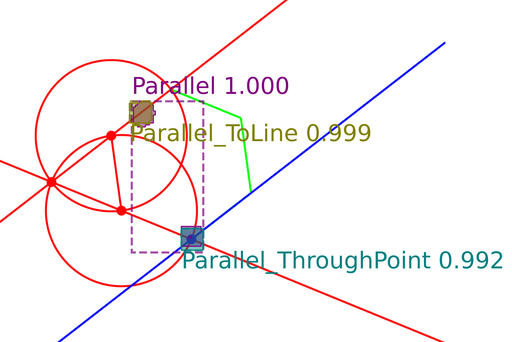
\includegraphics[scale=0.4  ]{img/Zeta-06_example/output_image4.png}}\\
\begin{small}
i) Step 4.\end{small} & \begin{small} j) Prediction for step 5. Based on this prediction a parallel line will be constructed.\end{small}\\

\subfloat{\includegraphics[scale=0.4  ]{img/Zeta-06_example/input_image5.png}} &
\subfloat{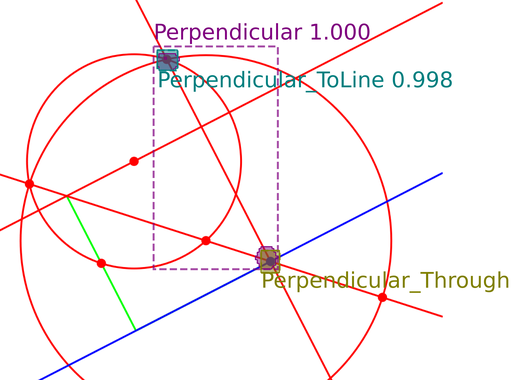
\includegraphics[scale=0.4  ]{img/Zeta-06_example/output_image5.png}}\\
\begin{small}
k) Step 5. The last parallel line constructed part of the goal, another side of the parallelogram.\end{small}&\begin{small}l) Prediction for step 6. Based on this prediction, a parallel line will be constructed. Note that there are two predictions of the parallel tool. Both of these parallels have to be constructed in order to finish the goal. In this step, detection with a higher Mask {R-CNN} score will be constructed.\end{small}\\

\subfloat{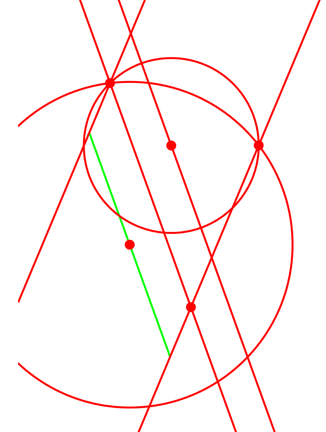
\includegraphics[scale=0.4  ]{img/Zeta-06_example/input_image6.png}} &
\subfloat{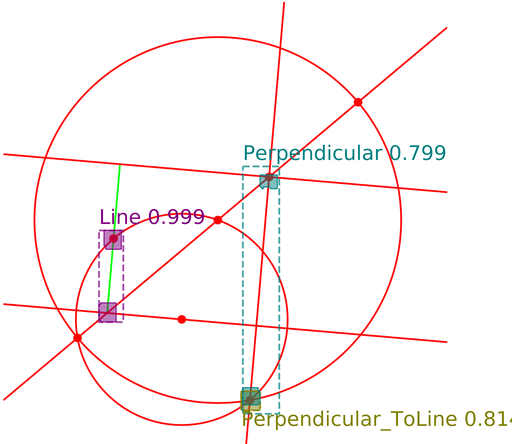
\includegraphics[scale=0.4  ]{img/Zeta-06_example/output_image6.png}}\\
\begin{small}
m) Step 6. The last parallel line constructed another part of the goal, one side of the parallelogram. \end{small}&\begin{small} n) Prediction for step 7. Based on this prediction, a parallel line will be constructed. Both predictions are still present. However, the prediction used in the previous step has a lower Mask {R-CNN} score. Hence, it is not used now.\end{small}\\

\subfloat{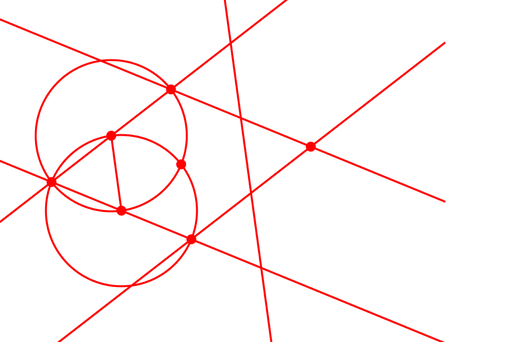
\includegraphics[scale=0.4  ]{img/Zeta-06_example/input_image7.png}}\\
\begin{small}
o) step 7. The last parallel line constructed the last part of the goal. Hence the geometric problem is successfully constructed.\end{small}\\

\caption{Example construction of level \textit{Zeta-12}: Parallelogram by 3 midpoints. The table contains 7 steps of the construction. Each step contains current progress on the left and Mask {R-CNN} prediction for a new step on the right. The green color denotes the goal and the red denotes the current state of the construction. Other colors mark prediction masks, bounding boxes, classes and scores for each detected object.}
\label{Zeta06_example}
\end{longtable}



\section{Motivation}
% - most existing work solve geometric constructions from known analytical models of individual primitives. The first motivation for this work is answering the question whether  whether geometric constructions can be solved given only the image input. 
% - this is similar to humans, which can ...

% - We wil show that the learnet recognizer is to some extent transferrable across different constructions and hence it opens up the possibility of using similar models hypothesis generators for automatic geometric theorem proovers [].

% - This project is a step towards developing methods that combine machine learning with machine reasoning over noisy visual (or visual and text [Seo15]) inputs. The long-term goal is developing automatic “virtual AI assistants” that can help mathematicians with complex proofs [Hales17] or reason about text and associated illustrations (e.g. automatic patent lawyer assistant). 
The first motivation for this work is to answer whether geometric constructions can be solved given only the image input. Most existing methods solve geometric constructions with knowledge of the analytical equitations behind each geometric primitive in the geometric problem.
\newline \newline
The second motivation is to develop a method that can solve geometric construction problems similar to how humans solve these problems. Since humans are capable of solving geometric problems without knowledge of the analytical model, moreover, we might have only a sketch that is an approximation of a geometrical problem. In this situation, we are forced to use only image data about the problem.
\newline \newline
The third motivation is a step towards developing an automatic geometric theorem prover. We will show that our learned recognizer is, to some extent, transferable across different constructions, and hence it opens up the possibility of using similar models hypothesis generators. This hypothesis generator can be used as an assistant for a human solver or a possible reinforcement learning method that will learn to combine proposed hypotheses.

%In some situations, we do not have an exact analytical model behind the scene. We might have only a sketch that is an approximation of a real-life problem. Furthermore, real-life problems cannot be precisely measured, and there is always some measurement error.  Input for our method is only an image of the scene with a highlighted goal. Our method's output is then a sequence of instructions on using the ruler and compass to construct the given problem. Our method's advantage is also that it provides hypotheses of construction steps, which might serve as an assistant for a human solver. Furthermore, the method's hypotheses proposal is generated with one forward pass through the neural network based on Mask {R-CNN}. Thus hypotheses are generated within a minute on a standard computer.
\section{Why is it difficult?}
In the course of the thesis we have to deal with four major problems: problem variability, construction ambiguity, object detection and training data generation. Figure \ref{variabilty_problem} is an illustration of the problem variability. The same geometric problem can have different variants, e.g.~different scale, rotation or different position of individual geometric primitives. Furthermore, each problem can be solved in an infinite number of ways. The most straightforward way to solve these problems is an exhaustive search of the construction space. The majority of existing methods use an analytical model to generate the next steps quickly. However, even with smart heuristics, a complete search of more complex problems can take up to days or even months of searching. Nevertheless, our goal is to play construction game Euclidea, so we aim to have a reasonable reaction time, but exhaustive search is often too slow.
\newline \newline
On top of that, we have to deal with object detection because only data about the geometric problem our method receives as input is an image. To recognize individual geometric primitives and their relative positions, part of our approach is object detection architecture. However, object detection architecture, such as Mask {R-CNN}, requires large amount of annotated data and computing time to be properly trained. Furthermore, training data have to be constructions that can be solved based on the image data. To train a model that can solve a geometric problem, we have to generate training data, which are constructions of multiple different configurations of the given problem. While creating new configurations of a problem, we have to create well-defined variants that are solvable. Problem variability, detection and data generation can be challenging apart, but we have to deal with them at once.
\begin{figure}[h!]
\begin{tabular}{cccc}
     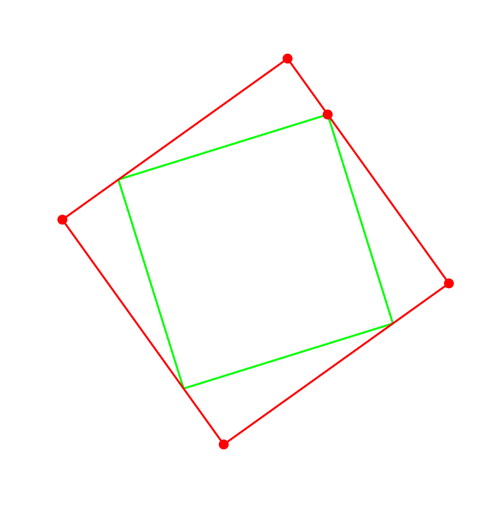
\includegraphics[width=0.2\textwidth]{img/problem_variability/problem_variability_1.png}
     &
     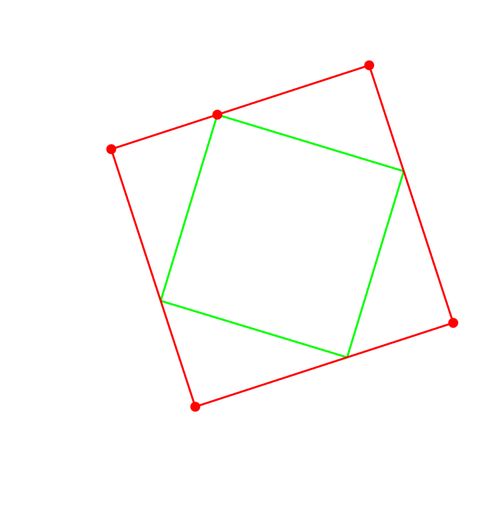
\includegraphics[width=0.2\textwidth]{img/problem_variability/problem_variability_2.png}&
     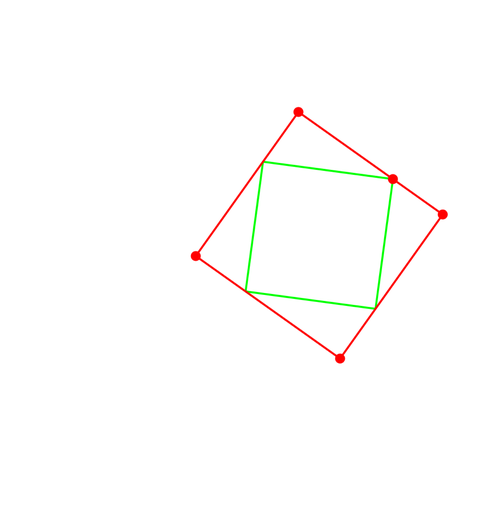
\includegraphics[width=0.2\textwidth]{img/problem_variability/problem_variability_3.png}
     &
     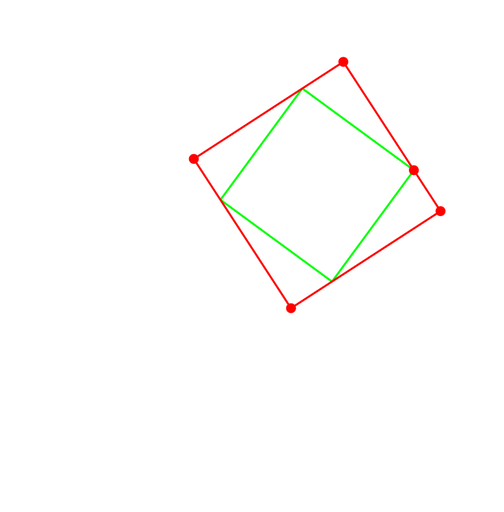
\includegraphics[width=0.2\textwidth]{img/problem_variability/problem_variability_4.png}
     \\
     a)  & b) & c) & d)
     \\
     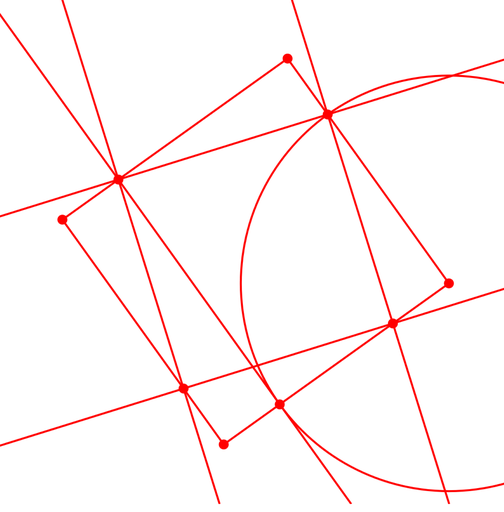
\includegraphics[width=0.2\textwidth]{img/problem_variability/problem_variability_1_solved.png}
     &
     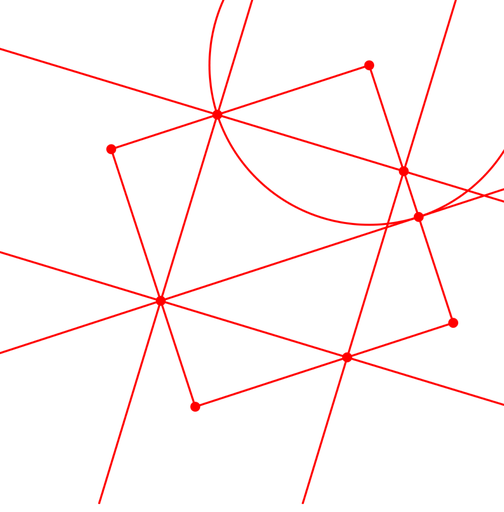
\includegraphics[width=0.2\textwidth]{img/problem_variability/problem_variability_2_solved.png}
     &
     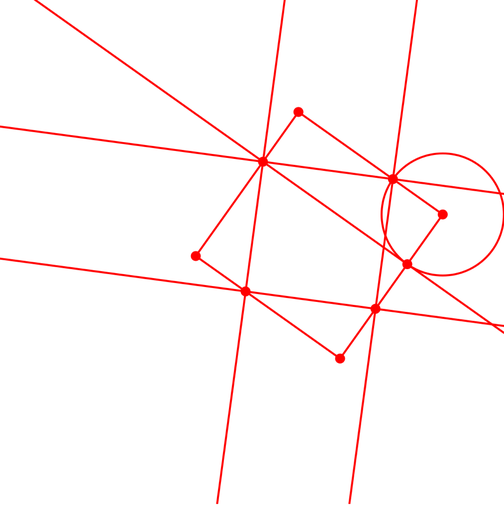
\includegraphics[width=0.2\textwidth]{img/problem_variability/problem_variability_3_solved.png}
     &
     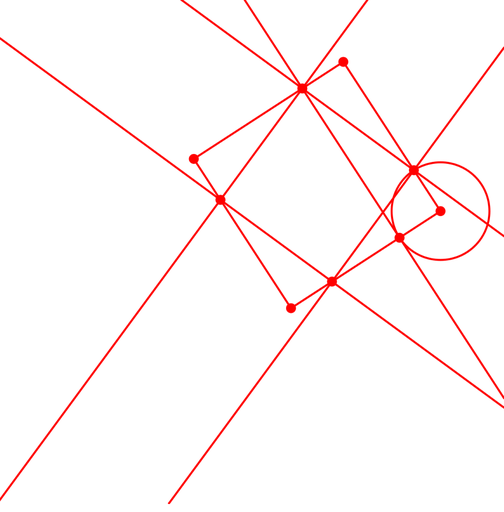
\includegraphics[width=0.2\textwidth]{img/problem_variability/problem_variability_4_solved.png}
     \\
     1) & 2) & 3) & 4)
     \\
\end{tabular}
\caption{Four instances of the same geometric problem, inscribe a square in the square when a vertex is given. Each instance contains a problem definition and a solution. In the top row are definitions of the problem and in the bottom row are corresponding solutions. Figures contains current states (red) d remaining goals (green).}
\label{variabilty_problem}
\end{figure}

\section{Related work}
Most geometric construction solvers utilize the analytical model for solving the problems. In our setup, we aim to find a solution to problems that we know are solvable. However, the focus of the research is also to prove or disprove the existence of a solution to a given problem. This proving process is also known as automated theorem proving (ATP). Methods of proving can be an exhaustive search for a solution \cite{ancient_problem}, by deriving new facts based on well-know properties in the problem or a combination of both \cite{botana15}. ATPs can also be solved with resolution theorem provers
and a coherent logic theorem provers \cite{stojanovicdurdevic:hal-01091011}. Alternatively, there are ATPs that can answer SAT-questions about geometric problems \cite{seo15}. For example, a question like: Based on known facts, are given lines perpendicular or not? On the other hand, some complex problems, such as Kepler conjecture, require assistance from ATP to be properly proven \cite{DBLP:journals/corr/abs-1211-7012} \cite{hales17}.
\newline 
In this thesis we combine ATP with an object detection architecture. One of the well-known architectures is the Mask {R-CNN} \cite{DBLP:journals/corr/HeGDG17}, which detects mask and bounding boxes in images and videos. This architecture is also used for pose estimation \cite{DBLP:journals/corr/abs-1712-09184}, \cite{Girdhar_2019_CVPR} or to estimate 3D motion and forces \cite{DBLP:journals/corr/abs-1904-02683}.

\section{Outline}
In Chapter \ref{euclidea_chapter}, we describe our implementation of Euclidea, an online construction game with an interface matching the desired agent. This chapter also describes how to generate new configurations of geometric problems used as training data for supervised learning. Then in Chapter \ref{chapter_exhaustive_search}, we analyze the difficulty of the problem by estimating the branching factor of the exhaustive tree search. In Chapter \ref{mrcnn_chapter}, we introduce a new approach based on Mask {R-CNN} as our primary model for supervised learning approach for the geometric construction problems. Then in Chapter \ref{chapter_unseen_levels}, we analyze the performance of Mask {R-CNN} models on the problems that were not seen during the training. To do so, we also describe the hypothesis tree search to search hypotheses obtained from multiple Mask {R-CNN} models. In the last Chapter \ref{experiment_chapter},
we describe multiple components of this model and experimentally demonstrate their benefits. Then we analyze the results of our best model on levels seen during the training. Then we analyze the accuracy of models for each level pack on unseen geometric problems with leave-one-out evaluation. Finally, we present multiple example solutions of Euclidea geometric problems.


\chapter{Euclidea environment for solving geometric construction problems}
\label{euclidea_chapter}
In this chapter, we describe Euclidea, an online geometric construction game. The game is played with construction tools, which are used to complete various geometric problems. We will then present our version of Euclidea and describe how to apply random transformations to existing levels to create new variants of the same level.

\begin{figure}[h]
\centering
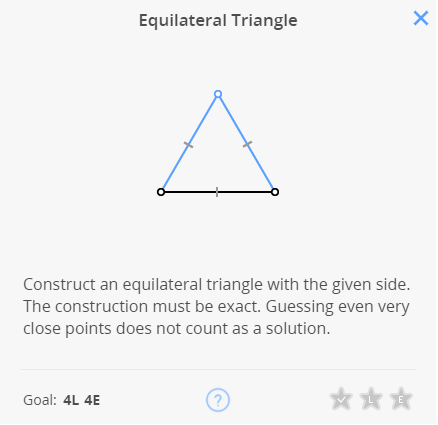
\includegraphics[width=70mm]{img/Actual_euclidea_definition.png}
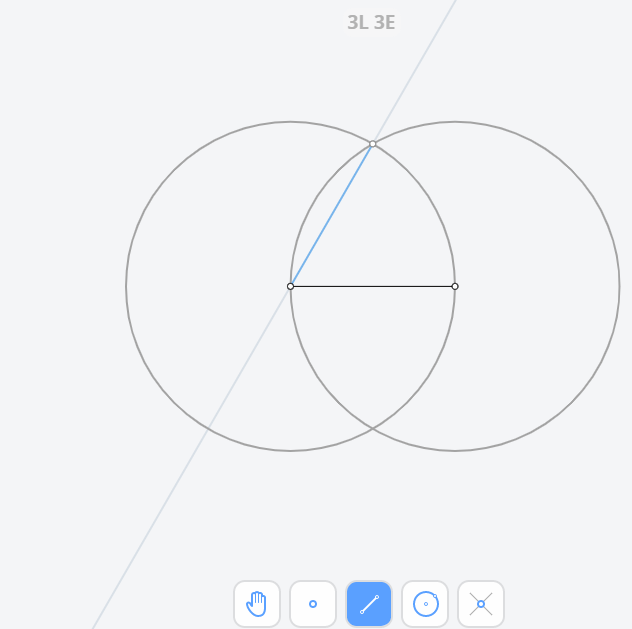
\includegraphics[width=70mm]{img/Actual_euclidea_screen.png}
\caption{Screenshot from Euclidea \cite{euclidea}. The goal of this level is to construct an equilateral triangle with the given side. The figure contains the goal description on the left and the construction on the right. The current state of the construction cost is 3L and 3E. Each usage of a tool costs pre-defined L cost and E cost. To get to the current state 3 tools were used: 2x Circle tool and 1x Line tool. Each tool costs 1L and 1E (see \ref{about_euclidea}).}
\end{figure}
\section{Euclidea}
\label{about_euclidea}
Euclidea is an online geometric construction game in 2-dimensional Euclidean space. In Euclidea we use the following terms:
\label{basic_concepts}
\begin{itemize}
    \item \textbf{Geometric primitives}  in Eculidea are points, lines and circles.
    \item \textbf{Level} in Euclidea is a geometric problem. Each level starts with an initial configuration, and the goal is to get to a target configuration.
    \item \textbf{Target configuration} denotes a state of a level that has all goals constructed, e.g.~it is done.
    \item \textbf{Goal description} is a definition of the remaining goals. In Euclidea, it is a visual information on how the remaining goal looks like. In our visualization marked as green lines, circles or points.
    \item \textbf{Current configuration} denotes a current state of construction, e.g~ it is initial configuration plus all constructed primitives with tools.
    \item \textbf{Initial configuration} denotes the first state of a level, and it also contains a goal description.
    \item \textbf{Scene}, \textbf{level instance} is generated by applying random transformations to the one predefined level template.
\end{itemize}
The main goal is to find a sequence of construction steps leading from an initial configuration of objects to a given target configuration. The construction steps utilize a set of straightedge and compass based tools (see Section \ref{euclidea_tools}). The game has two additional goals (L and E) and one hidden goal (V). The additional goals are to minimize L or E costs. The L cost is 1 for each tool used, with the exception of Point, Move, and Intersection tools, which have zero cost. The E cost equals the number of lines and circles necessary to construct the tool. The hidden goal is to find all possible solutions to a level and is thus available only for levels with multiple solutions.
\newline \newline
Every tool takes up to 3 arguments with values specified by coordinates of clicks on the image of the scene, for example, $circletool(A, B)$, where $A$, $B$ are points on the image of the scene. An exception is the Move tool, which is realized by dragging points to another place, although it can be represented also by a translation vector, defined by two click coordinates.
\newline \newline
Euclidea is divided into 15 level packs (Alpha, Beta, Gamma, \dots, Omicron) with increasing difficulty. Each level pack contains around 10 levels with a similar focus. Description of levels from Alpha to Zeta can be found in Appendix \ref{appendix_ch1} see Table \ref{level_descriptions}.
\section{Precision and goal evaluation}
\label{euclidea_precision}
In Euclidea, each level has its analytical model, which is projected on an image canvas. Each pixel in the image thus corresponds to a point in the analytical model. However, the analytical model points have float coordinates, making it impossible to find out precise coordinates of a point in the analytical model based on image data. Euclidea therefore provides certain tolerance for clicks and automatically finds the nearest geometric primitive corresponding to the click coordinates. 
\newline \newline
Euclidea checks the goal on the analytical level, so the player cannot cheat by drawing a similar goal instead. The player has to construct the target configuration to ensure that the result is the same as the goal.
\newline
\newline
In practice, the float parameters of two same geometric primitives stored in different objects cannot be the same, so even this comparison has some tolerance. We have to keep this float tolerance in mind because it might cause issues, as described in the chapter about data generation (see Section \ref{data_generation}).
\section{Tools}
\label{Euclidea_tools}
This section describes the tools available in Euclidea. They can be divided into 3 categories: Tools creating points, construction tools for lines and circles and the Move tool.
\label{euclidea_tools}
\subsection{Point and Intersection tools} \label{point_tool}
The Point tool takes one argument and creates a point in the desired location. However, in accordance with the precision approach in Euclidea (see Section \ref{euclidea_precision}), this tool also finds all line and circle primitives within a small neighborhood of the click coordinates and creates a point using the first applicable rule from the following:
\begin{enumerate}
  \item Create a point on the closest intersection of primitives if there are any.
  \item Create a point on the closest geometric primitive if there are any.
  \item Create a point at the exact coordinates given by the argument.
\end{enumerate}
\newline \newline
The Intersection tool creates points on all intersections of the two geometric primitives given in arguments. 
Both tools have E and L costs equal to 0.

\subsection{Construction tools}
The following tools take several arguments. Before a tool is executed, each click coordinates in the arguments are assigned the nearest geometric primitive matching the argument type.
\begin{table}[!htb]
\begin{center}
 \begin{tabular}{| m{2.7cm}| m{3.8cm} | m{5.2cm}| c{0.5cm} | c{0.5cm} |} 
 \hline
 \bfseries Tool &
 \bfseries Arguments &
 \bfseries Description & \bfseries L  &
 \bfseries E  \\
 \hline
 Line &
 (point, point) &
 Draw a line passing through the given points. &
 1 & 1 \\
 \hline
 Circle &
 (point, point) &
 Draw a circle centered at the first point with a radius marked by the second point.
 & 1 & 1 \\
 \hline
 Perpendicular Bisector &
 (point, point) &
 Draw the perpendicular bisector of two given points. & 1 & 3 \\
 \hline 
 Angle Bisector &
 (point, point, point) &
 Draw the axis of an angle, where the second point marks the vertex and the first and the third points lie on its rays. &
 1 & 4 \\
 \hline
 Perpendicular &
 (line, point) &
 Draw a line perpendicular to the line passing through the point. &
 1 & 3 \\
 \hline
 Parallel &
 (line, point) &
 Draw a line parallel to the line passing through the point. & 1 & 4 \\
 \hline
 Compass &
 (point, point, point) &
 Draw a circle with a center in the third point and a radius given by the distance between the first two points. &
 1 & 4 \\
 \hline
 %Intersection &
 %(line or circle, line or circle) &
 %Create points on all intersections of the two given geometric primitives. & 0 & 0\\
 %\hline
\end{tabular}
\caption{Tools available for construction steps in Euclidea. L and E denote the tool costs (see Section \ref{about_euclidea}).}
\end{center}

\end{table}

\subsection{Move tool}
\label{move_tool_definition}
The Move tool does not add any new geometric primitive but instead moves one primitive elsewhere and then recomputes the whole analytical model, if necessary. For example, if we move a line, the Move tool must also move all points on that line. Furthermore, it also has to adjust all the primitives intersecting those points, and so on. In Euclidea, the Move tool is used for exploring and understanding a given level. However, each level specifies the set of movable primitives, so not every primitive can be moved.
\newline
\newline
If a level configuration has multiple solutions, moving the primitives might remove some of the solutions. We will discuss this problem in data generation (see Section \ref{data_generation}).

\section{Our Euclidea-like environment}
In this thesis, we use our python version of Euclidea based on \cite{py_euclidea}, which contains every level and implements every tool.

\section{Example construction}
\label{euclidea_vizualization}
Each state in our environment is represented by two gray-scale images: the current configuration and the target configuration. The two images are stacked into an RGB image, where the red channel is the current state, and in the green are remaining goals, and the blue channel is filled with zeros. 

Figure \ref{EuclideaExample} shows an example of a level in our environment and the construction steps. The task of the level is to construct an equilateral triangle given by one side.

\begin{figure}[h!]
\begin{tabular}{ll}
\subfloat{\includegraphics[width = 2.6 in]{img/Equilateral_example/input_image0.png}} &
\subfloat{\includegraphics[width = 2.6 in]{img/Equilateral_example/input_image1.png}}\\

 a) Initial configuration & b) Construction step:1 \\

\subfloat{\includegraphics[width = 2.6 in]{img/Equilateral_example/input_image2.png}} &
\subfloat{\includegraphics[width = 2.6 in]{img/Equilateral_example/input_image3.png}}\\

c) Construction step: 2 & d) Construction step:3 \\
\subfloat{
\includegraphics[width = 2.6 in]{img/Equilateral_example/input_image4.png}}
&
%\subfloat{\includegraphics[width = 2.6 %in]{img/Equilateral_example/input_image5.png}}
\\

e) Construction step: 4 - level finished&  \\


\end{tabular}
\caption{Construction steps in our version of Euclidea for level \textit{Alpha-05}: Equilateral Triangle. Current state (red) and remaining goals (green). The first state is the level definition. In each step, we use one tool to construct the goal. Note that in Euclidea, we can see the goal, but we cannot use it for construction.}
\label{EuclideaExample}
\end{figure}

\section{Generation of level instances} \label{data_generation}
\label{data_gen_ref}
To train an automatic recognizer, we add a generator of new level instances to our version of Euclidea. The new scenes are based on predefined ones. Each level has one predefined scene and goal definition. In order to generate a new scene, we transform the predefined scene using the Move tool (see Section \ref{euclidea_tools}). Generated scenes can be either valid or degenerated. Degenerated scenes cannot be solved due to precision problems or other construction problems. We will describe how to recognize degenerated scenes in the rest of Section \ref{data_generation}.
\newline \newline
We use the following steps to generate training data:
\begin{enumerate}
  \item Load predefined scene.
  \item Apply random rotation.
  \item Randomly move all movable points.
  \item Apply random scale. 
  \item Check scene validity / degeneration.
  \item Apply random translation.
\end{enumerate}
There are two types of geometric primitives in the predefined scenes: constrained and movable. Constrained objects are constrained to another geometric primitive in the scene. We denote a construction of each constrained object as a ``step''. Objects constructed within one step can be constrained to any movable object or to an object constructed in previous steps.
An example of a constrained object is: ``point on a line'', ``line perpendicular to another line'' etc.
Movable objects on the other hand are not constrained to any other object, so they can be moved, but their movement also moves all other objects constrained to them. Our version of Euclidea contains only movable points. Circles and lines may be constrained to other points; note that these points can be hidden from the visualization of the level.
\newline \newline
The generation process can lead to degenerated scenes, i.e.~scenes that cannot be solved based on image information, mainly because certain parts are too close to each other and cannot be distinguished. Additionally, during re-scaling, we compute a minimal possible scale to avoid small scenes degenerated due to a small size.
 
\subsection{Degeneration criteria}
\label{degen_criteria}
Degeneration criteria are a set of rules that attempt to determine whether a scene is degenerated. 
We use the following four rules:
\begin{enumerate}
  \item Different points cannot be too close to each other, measured in pixels.
  \item Circles cannot have a too small radius, measured in pixels. 
  \item Two lines with a similar cannot be too close. Normal vectors compared in the analytical model.
  \item Intersections of geometric primitives can not be too close to points used in the construction, measured in pixels.
\end{enumerate}
The Rule 4. was added later as it is mainly used in the advanced Euclidea levels.
Rules number 1.-3.~were at first only applied to geometric primitives that were in the level definition. However, the degeneration status of a level definition does not include the degeneration of construction. So construction degeneration has to be checked as well. There is possibly an infinite number of different constructions, and we cannot make them all valid. 
\newline \newline
Without rule 4.~the degeneration criteria had two significant problems that led to degeneration:
\begin{itemize}
  \item Levels with multiple solutions can have configurations that make those solutions coalesce into each other. Probability of this generation goes to $0$, but those solutions can be so close together that we cannot differ one from another based on visual information.
  \item During construction, we create many intersections between geometric primitives. Although we force points created during construction to be reasonable by previous rules, we force only those points that are necessary for the construction. Sometimes a point not necessary for the construction can be too close to a construction point.
\end{itemize}
The second problem is more general than the first one, and the solution to it also solves the first problem. To realize rule 4.~we go through all intersections between all pairs of primitives and check if they are far enough from important points.
\newline \newline
As we found out, for some levels these degeneration rules do not ensure validity and we need to define level-specific degeneration criteria as described next.  

\subsection{Level-specific degeneration criteria}
Certain levels require degeneration rules that are not general. Some definitions of the levels also have ``additional degeneration'' which is again a set of rules applied only for instances of that level. The most frequent use of those additional degeneration rules is that specific angles cannot be too small or obtuse. It is also used to add additional constraints between objects of the scene that are level-specific. For example, in one level that contains two squares, those squares should not overlap.
\subsection{Precision problems}
While generating data, especially the constructions, we also have to deal with precision problems tied with scene re-scaling.  Generally, when we create a construction, we have to check whether two primitives are the same.  Each primitive is defined by a number of normalized arguments. An object with parameters $args_1$ is identical to an object with parameters $args_2$ when:
\begin{equation}
|args_1 - args_2| < \epsilon
\end{equation}
However, the difference can surpass $\epsilon$ when the objects are upscaled. Then objects are considered the same, but they are not. This can also occur the other way around. This may generate different construction then then desired. This precision problem has to be dealt with during the construction creation. However, it is only present when a level can have multiple solutions that can be potentially very close.

\chapter{Complexity of exhaustive search for constructions}
\label{chapter_exhaustive_search}This chapter analyzes the difficulty of exhaustive search for geometric constructions in Euclidea. We analyze the exhaustive search by computing the branching factor of the tree search. After defining our choice of tree search, we analyze the branching factors in the actual tree search.
\newline \newline
The Euclidean space has an infinite number of constructions. Hence the tree search for possible solutions has to have a large branching factor, and the search problem is unsolvable within a reasonable time to play the Euclidea game.
According to \cite{ancient_problem}, exhaustive search can be done within days on a standard computer. This chapter is an illustration of how difficult the problem is.

\section{Euclidea tools for tree search}
\label{tools_for_treesearch}
Before we decide which variant of the tree search to use, we will describe how to generate new nodes. We will use geometric primitives instead of click coordinates as the tool arguments. All tools can work with geometric primitives. The only exception is the Point tool. As a reminder, the Point tool creates points on intersections or primitives or points in open space (see Section \ref{point_tool}). For search purposes, we can use the Intersection tool for finding intersections instead. The creation of a point on a geometric primitive is even more straightforward with the primitive given as the argument. However, there is possibly an infinite number of choices to create a point on the geometric primitive. We will only create random points that are ``reasonable''. A reasonable point is a point that is not too close to any other point nearby. We will omit the function for open space point creation of the Point tool and not use it at all. That function may be needed to construct some more advanced levels in Euclidea, but in this chapter, we will investigate the complexity of solving only simple levels of the Euclidea game.

\section{Estimate of the branching factor}
\label{degrees_of_freedom}
A complete tree search in the worst case has to go through $b^n$ possibilities, where $b$ is the branching factor, and $n$ is the minimal depth of the solution. We can thus analyze the difficulty of the search problem by estimating the branching factor.
\newline \newline
For this purpose, we have to define the number of degrees of freedom (\DOF{}) of each tool. \DOF{} is determined by the number of different tool outputs given by permutations of the arguments. For example the Line tool has \DOF{} = 1, since $line(A, B) = line(B, A)$, whereas the Circle tool has different outputs \newline$circle(A, B) \neq circle(B, A)$ hence circle has \DOF{}  equal to 2. The highest value of \DOF{} is 3 (Compass and Angle Bisector tools).
\newline \newline
\label{estimate_of_branching_factor}
For the purposes of the estimate, let us define $G$ as the number of geometric primitives in the current scene. Then we can divide the tools into 3 groups, according to the number of arguments and the \DOF{}:
\begin{itemize}
    \item \textbf{Line, Perpendicular Bisector, and Intersection} tools have 2 arguments and a sing1e degree of freedom. Each tool in this group adds the same number of branches, which can be computed as follows:
    \begin{equation}
    G + {G \choose 2} = \frac{1}{2}G^2 + \frac{1}{2}G,
    \end{equation}
    $G$ branches for each tool usage like $\linetool(A,A)$ and ${G \choose 2}$ for each tool usage like $\linetool(A,B)$, where $A$,$B$ are unique combinations. 
    \item \textbf{Circle, Perpendicular, and Parallel} tools have 2 degrees of freedom and 2 arguments. Each tool in this group adds the same number of branches, which can be computed as follows:
    \begin{equation}
    G + 2{G \choose 2 } = G^2.
    \end{equation}
    This group has maximal possible \DOF{} for its number of arguments, therefore $G^2$.
    \item \textbf{Angle Bisector and Compass} tools have 3 degrees of freedom and 3 arguments. Each tool in this group adds the same number of branches, which can be computed as follows:
    \begin{equation}
    G + 4 {G \choose 2} + 3 {G \choose 3} = \frac{1}{2}G^3 + \frac{1}{2}G^2 , 
    \end{equation}
    $G$ branches for each tool usage like $\compass(A,A,A)$. $4{G \choose 2}$ counts the number of each tool usage like $\compass(B,A,A)$ and ${G \choose 2}$ gives the number of combinations we can pick in 2 ways which argument is used twice an in 2 ways we can order arguments (\DOF{} = 3, but -1 since two parameters are same). $3{G \choose 3}$ branches for each tool usage like $\compass(A,B,C)$, times 3 because \DOF{} is equal to 3.
\end{itemize}
The worst case happens when all tools are allowed. The branching factor is then the sum of branches of each tool:
\begin{equation}
b =  G^3 + \frac{11}{2}G^2 + \frac{3}{2}G.
\end{equation}


Note that the number of geometric primitives grows with every successful use of any tool by at least +1. Furthermore, for the Intersection tool we can create 2 points if we use the tool to find the intersection of two circles.
\newline \newline
If we assume that every tool is allowed and there is one primitive at the beginning, then when we add 1 primitive at each step, the branching factor estimate grows as follows (see Table \ref{estimate_growth}).
\newline \newline
\begin{table}[h]
\resizebox{.95\textwidth}{!}{
\begin{tabular}{l|rrrrrrrrr}
    %\centering
     \# of primitives & 1 & 2 & 3 & 4 & 5 & 6 & 7 & 8 & 9
    \\ \hline
     branching factor estimate & \textbf{8}&\textbf{33}&\textbf{81}&\textbf{158}&\textbf{270}&\textbf{423}&\textbf{623}&\textbf{876}&\textbf{1188} \\

\end{tabular}}
    \caption{Growth of the branching factor estimate (see Section \ref{degrees_of_freedom}). Each step adds one geometric primitive.}
    \label{estimate_growth}
\end{table}
\newline \newline
%\[\textbf{8 - 29 - 69 - %134 - 230 - 363 - 539 - %764 - 1044}\]

However, these branching factors estimates represent the worst-case scenario and some of the actions can be invalid in the Euclidea environment. We can decrease the branching factor by simple heuristics. We will describe these heuristics in the next section.


\section{Tree search over known primitives}
\label{tree_seach}
With changes to tools in the previous section (see Section \ref{tools_for_treesearch}), we can use any type of tree search on our problem. Although we omit creating random points in space, we can solve several levels, especially in the first level pack of Euclidea.
\newline \newline
In theory, we can use any tree search algorithm. However, the iterative deepening makes the most sense for its memory usage. Additionally, the levels construction length is known, so the initial depth can be set to the length of the construction, effectively transforming iterative deepening to depth-first search.
\newline \newline
To reduce the branching factor of the tree search, we use several heuristics. Amongst them are 2 heuristics preventing action repeats, but most notably, the following two heuristics:
\begin{itemize}
    \item \textbf{Reward cutting}:  It is beneficial to know the effect of an action to decide which action will be used first. To get the results of actions, we execute each action and then reverse it. This can reveal errors that can occur during action execution. Most importantly, it allows us to check if an action completes a part of the goal. If it does, we assume this action is the only action in the current node of the search.
    \item \textbf{Goal construct-ability}: Since we use iterative deepening, the maximal depth is equal to $d$. If we are in depth $d-i$ and there are still $k$ parts of the goal to complete, and $k > i$, we can cut the branch since we cannot finish the goal in $i$ steps.
\end{itemize}
We can use the search to analyze the complexity of geometric construction problems. However, the search often runs longer than desired to play the game.
\begin{table}[h!]
    \centering
    \resizebox{.95\textwidth}{!}{

    \begin{tabular}{|c|c|c|}%
    \hline
    \bfseries Alpha levels & \bfseries Successful search & \bfseries Branching factor (estimate)
    \csvreader[head to column names]{../img/tables/alpha_branching_factors.csv}{}% use head of csv as column names
    {\\\hline\level\ & \suc & \shortstack{\\ \branch \\ (\estimate) \\} }% specify your columns here
    \\\hline
    \end{tabular}
    }
    \caption{Branching factors of Alpha levels, first 10k nodes visited. The first column show Euclidea level. The second column indicates whether the search completed the construction successfully (True/False). The third column gives the average branching factor (top) at each depth of the search and its estimate in the parenthesis (bottom).}

    \label{alpha_branching}
\end{table}
\begin{table}[h!]
    \centering
\resizebox{.95\textwidth}{!}{

\begin{tabular}{|c|c|c|}%
    \hline
    \bfseries Gamma levels & \bfseries Successful search & \bfseries Branching factor (estimate)
    \csvreader[head to column names]{../img/tables/gamma_branching_factors.csv}{}% use head of csv as column names
    {\\\hline\level\ & \suc & \shortstack{\\ \branch \\ (\estimate) \\} }% specify your columns here
    \\\hline
    \end{tabular}
    }
    \caption{Branching factors of Gamma levels, first 10k nodes visited. The first column show Euclidea level. The second column indicates whether the search completed the construction successfully (True/False). The third column gives the average branching factor (top) at each depth of the search and its estimate in the parenthesis (bottom).}
    \label{gamma_branching}
\end{table}
\newline \newline
In the easier levels, the heuristics allow us to reduce the branching factor significantly. However,
for more complex levels, the measured branching factor approaches the estimate given in Section \ref{estimate_of_branching_factor}.
\newline \newline
Tables \ref{alpha_branching} and \ref{gamma_branching} show the branching factors of level packs Alpha and Gamma, respectively.
Branching factors of the other level packs can be found in Appendix \ref{additional_branching_factor_tables}.

\section{Tree search over automatically recognized primitives}
The search described in Section \ref{tree_seach} assumed that the geometrical primitives in the environment were known. This assumed having access to the environment. Since this thesis aims to construct geometric constructions from image data, we also modified the iterative deepening to automatically detect and recognize geometric primitives in the image and then proceed with the search with these detected primitives. We use the Mask {R-CNN} network trained to recognize all geometric primitive in the scene. To train the network, we use Alpha levels, where each target is a mask of all geometric primitives in the scene. We discuss more in-depth details of the Mask {R-CNN} object detector in the next chapter. This approach rapidly slows the deepening because we have to generate an image of the scene and then run the CNN detection in each node. This can be further optimized to run the detector only once at the beginning of the search, and then newly constructed geometric primitives can be derived based on the difference between the previous state image and the current state image. Overall, this approach is a slower variant of the previous tree search, but it fits the theme of the thesis.
\chapter{Supervised learning approach}
\label{mrcnn_chapter}
In this section we introduce Mask {R-CNN} \cite{DBLP:journals/corr/HeGDG17} as our primary supervised model for solving Euclidean construction problems, describe how to train it and how to obtain Euclidea actions from Mask {R-CNN} model predictions.

\begin{figure}[h]
\centering
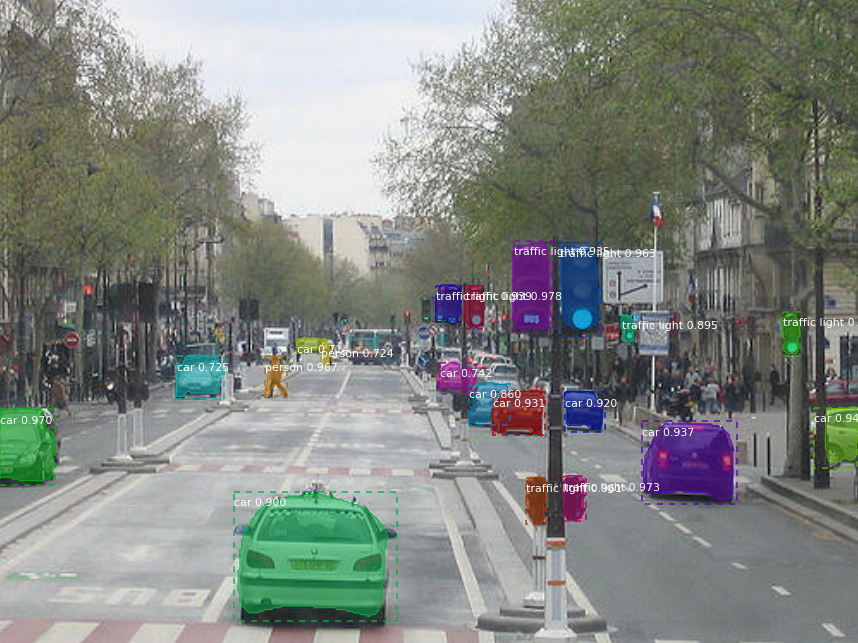
\includegraphics[width=140mm]{img/mask_rcnn_example.png}
% Rozměry také není nutné uvádět.
\caption{Example of a detection with the Mask {R-CNN} model. Source: \cite{matterport_maskrcnn_2017}}
\label{mrcnn_example}

\end{figure}


\section{Mask {R-CNN}, review}
Mask R-CNN is a deep neural network used for, detection, classification and segmentation of objects in images and videos. The input is an image and the output is a set of bounding boxes, segmentation masks and class labels for each detected object instance in the image. Example output is shown in Figure \ref{mrcnn_example}
\newline \newline
Mask {R-CNN} first computes image features with a convolutional backbone, usually the ResNet backbone. Followed by two stages of Mask {R-CNN}. The first stage is a deep convolutional network with Region Proposal Network, which proposes regions of interest from the features computed by the backbone. The second stage uses the ROI pooling layer and predicts class, bounding box and mask for each ROI.

\begin{figure}[h]
\centering
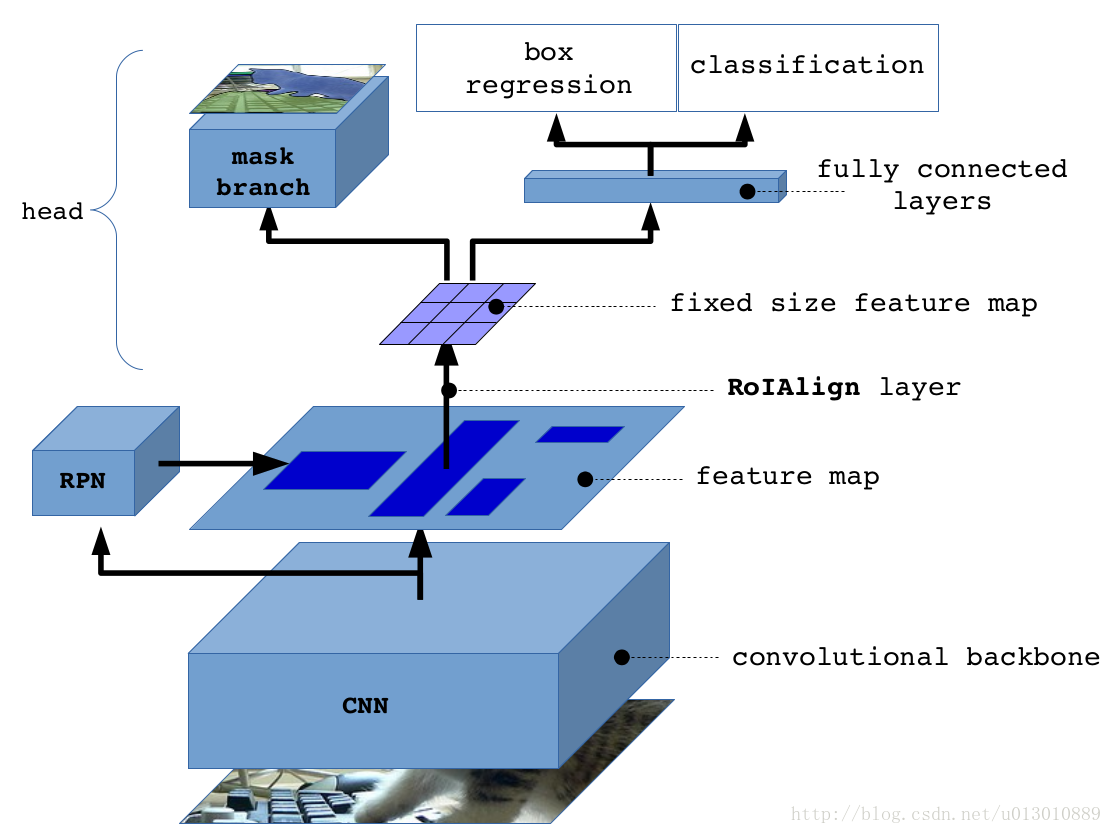
\includegraphics[width=140mm]{img/mask-rcnn_schema.png}
\caption{Diagram of the Mask {R-CNN} model, the CNN backbone, the ROI proposal network and head mask layers. Source: \cite{mrcnn_schema}}
\label{mrcnn_example}

\end{figure}
\section{ Mask R-CNN for solving geometric constructions}
In Figure \ref{our_approach_schema} we can see the schema of our approach. We generate the training data as we go through Euclidea levels. We solve levels by following a predefined construction that is recomputed to a current instance in the generation process (see Section \ref{degen_criteria}). Each application of a Euclidea tool corresponds to one sample in the training data. To train Mask {R-CNN} to solve geometric constructions, we have to create training data that represent tool usage, and we have to adjust outputs of the network to work with the Euclidea-like environment. 
\newline \newline
We denote each application of a tool in our environment as an ``action''. For this purpose, we assign each tool an index, e.g.~ 1 for Line tool, 2 for Circle tool, etc. An action is then represented by the index of the tool and the corresponding number of click coordinates (see Section \ref{Euclidea_tools}). For example, the Line tool needs two action clicks, which represent two points on the line. Next, we will describe how to generate training data for Mask {R-CNN} and how to infer actions from those masks. 
\begin{figure}[h]
\centering
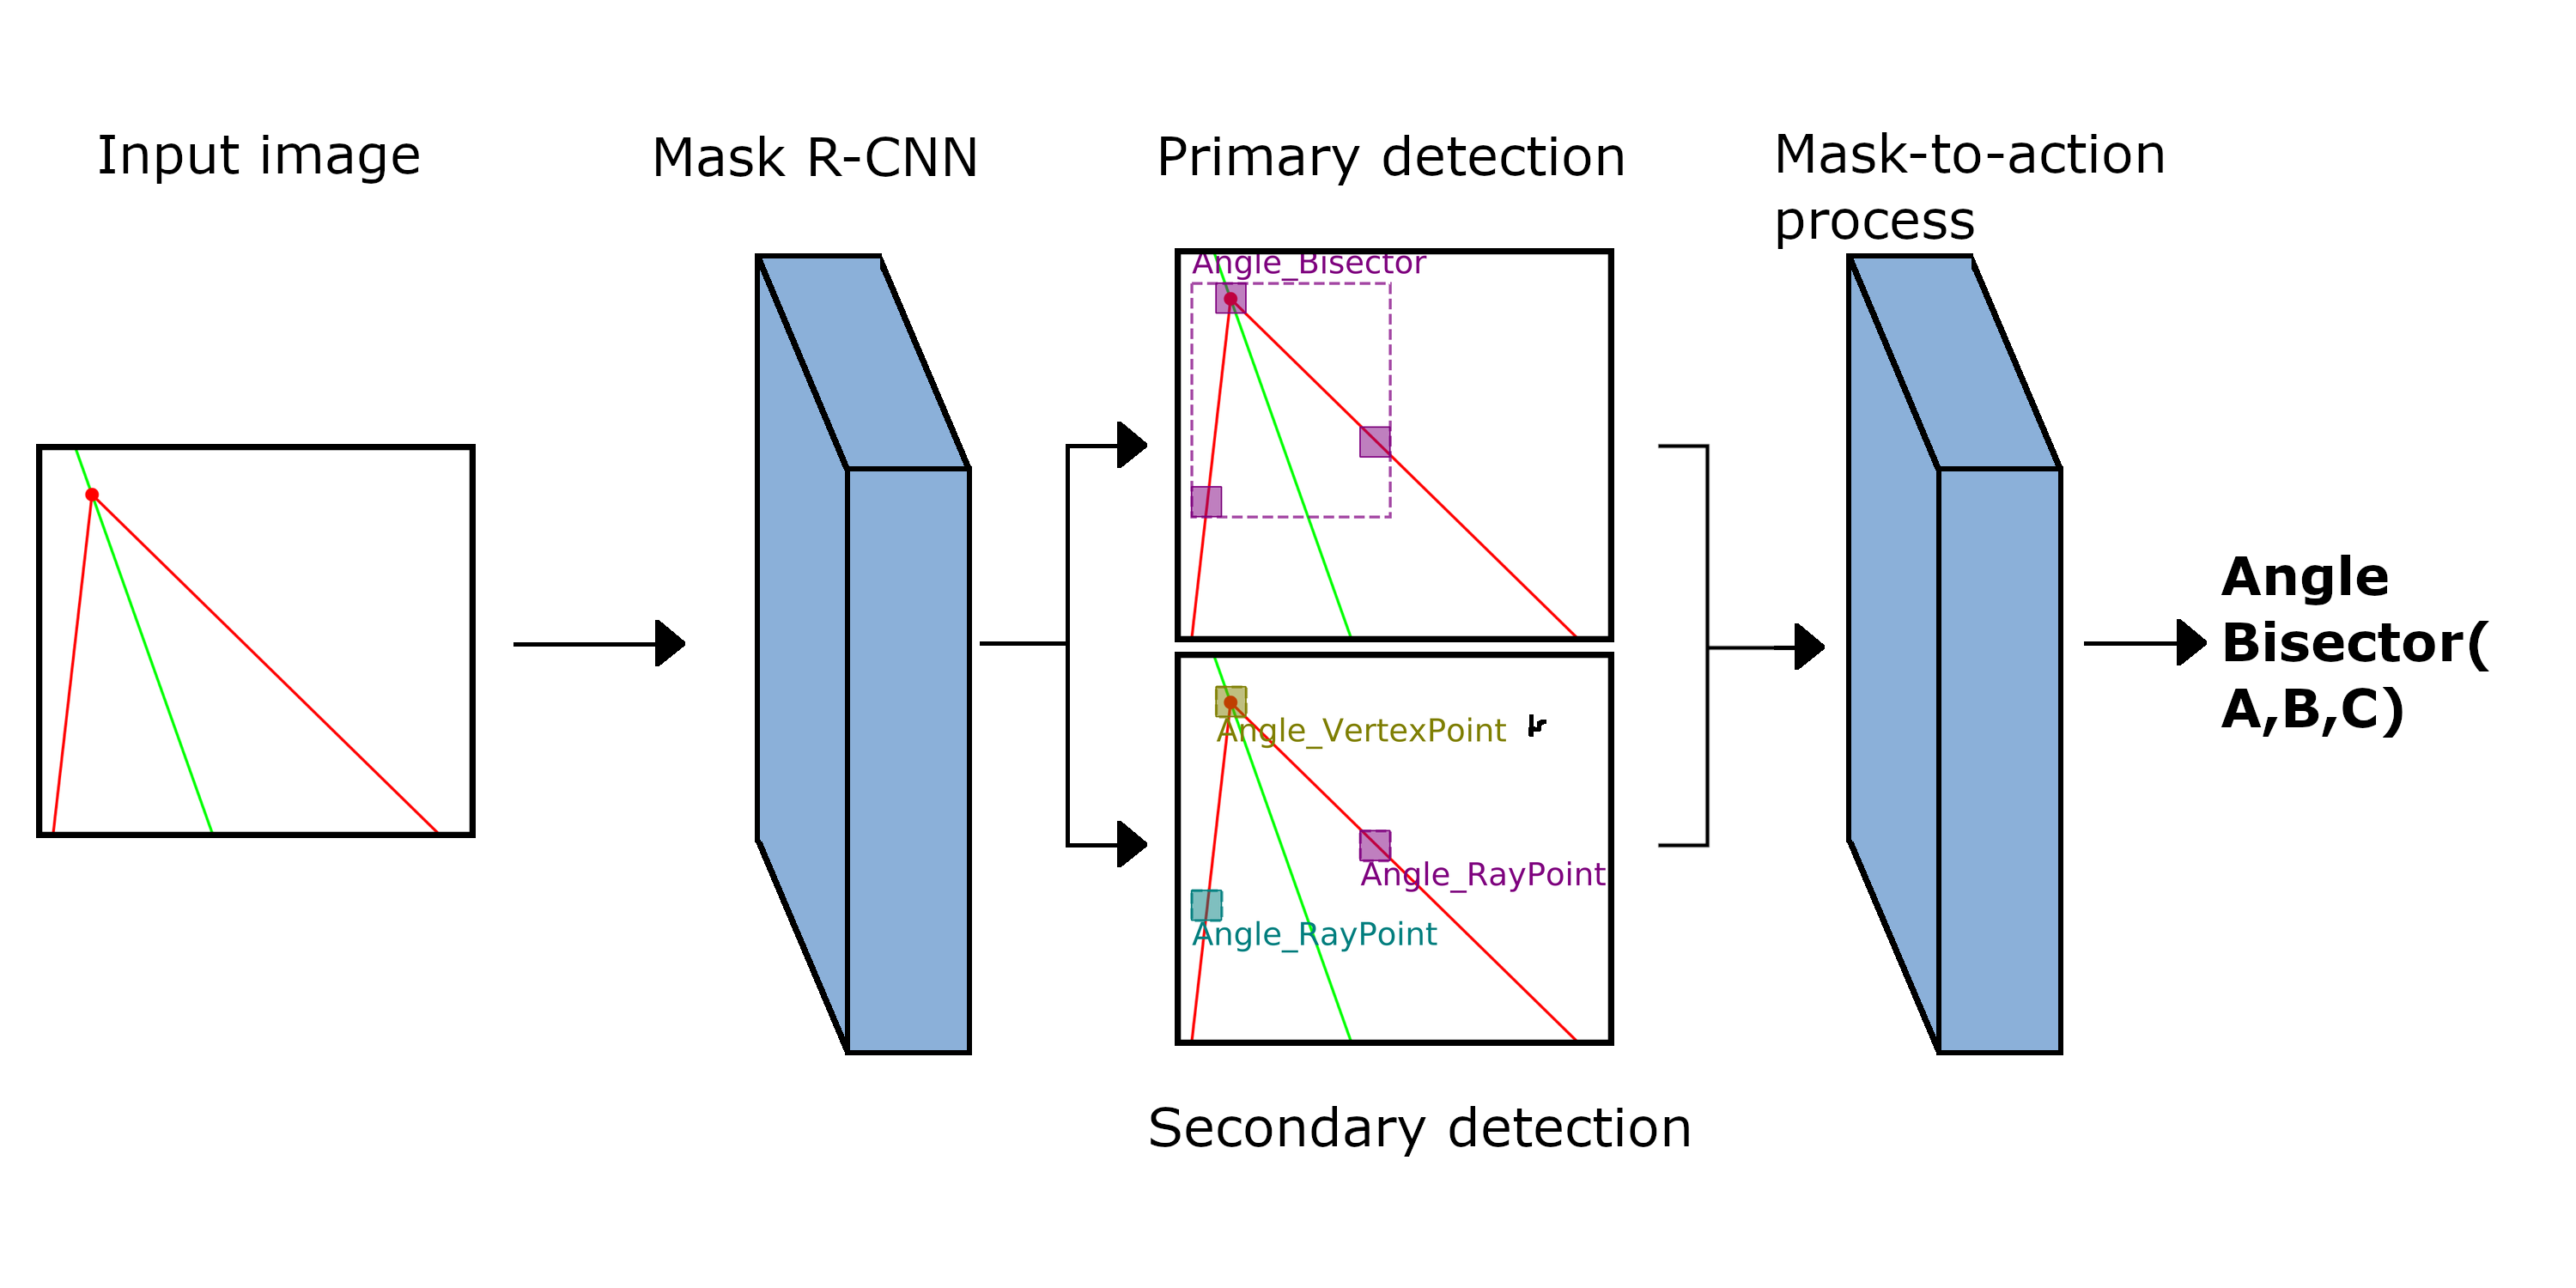
\includegraphics[width=140mm]{img/approach_schema.png}
\caption{Diagram of our approach. The input is an image of the scene, which is run through Mask {R-CNN}. The input image contains an RGB image with the current state of the construction in the red channel and the remaining goal in the green channel. The results are primary and secondary detections, which are then used to obtain an action tool for Euclidea. Note that there is no head for predicting primary and secondary detections. Instead, both are predicted with the same head and sorted to primary and secondary detections by the prediction id. How the Mask-to-action process works is described Sections \ref{action_to_mask} and \ref{position_dependent_pars}}
\label{our_approach_schema}

\end{figure}
\subsection{Action to mask}
\label{action_to_mask}
\begin{figure}[h]
\centering
\begin{tabular}{c c}
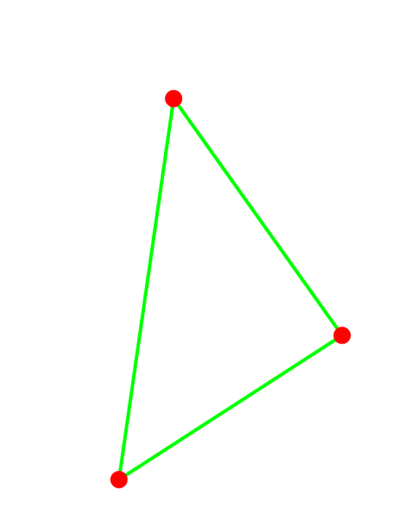
\includegraphics[width=0.45\textwidth]{img/ExampleTrainingData/01_01_input.png} &
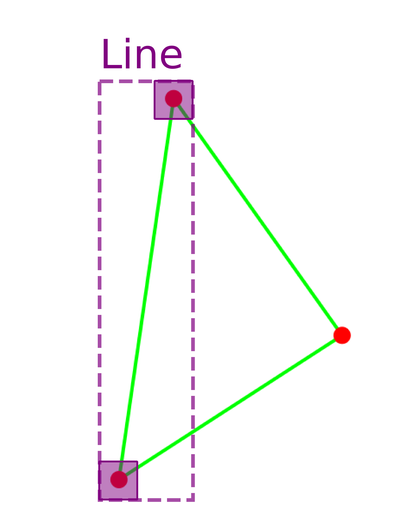
\includegraphics[width=0.45\textwidth]{img/ExampleTrainingData/01_01_primary.png} \\
a) Input & b) Primary detection
\end{tabular}
\caption{A sample from training data for level \textit{Alpha-01}: Tutorial for the Line tool, connects points. Both parts contain the current state (red), remaining goal (green).
Input for the model is on the left and target mask (purple in this case) for the Line tool with respective bounding box on the right. The mask contains two areas for each endpoint of the triangle side, representing click coordinates for the tool. The Line tool does not have position-dependent parameters. Hence the secondary detection is empty and not shown.}
\label{training_data_primary_01_01}
\end{figure}
We represent the input of the Mask {R-CNN} as an image of the scene with current state in the red channel and the remaining goal in the green channel. In our experiments, we also add extra channels representing history (see Section \ref{history_channel}). The $n$-th history channel represents the state of the scene $n$ steps before the current state.
\newline \newline
A target is a pair of an object type and its location, represented as a mask of the object. Object type corresponds to the tool that is used in the step. The target mask is the mask of each point click contained in the step.
These sub-masks are squares around the click location. Also, some tools have a line as its argument; passing a line argument can be a mask of a single click on the line or a mask of the whole line. Figure \ref{training_data_primary_01_01} shows an example of input and output.

\subsection{Tools with position-dependent parameters}
\label{position_dependent_pars}
\begin{figure}[h]
\centering
\begin{tabular}{c c c}

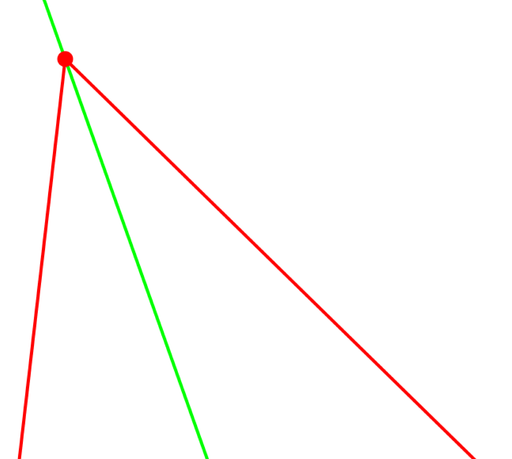
\includegraphics[width=0.3\textwidth]{img/ExampleTrainingData/02_02_input.png} &
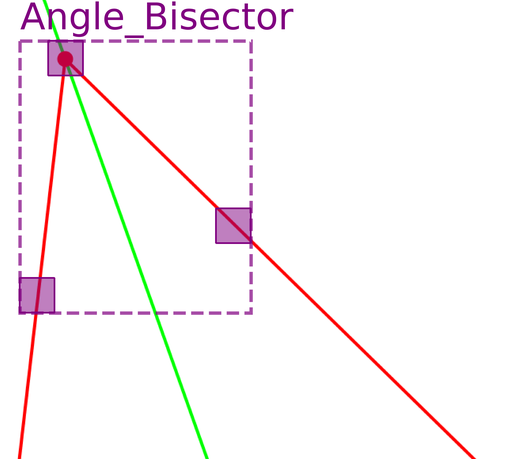
\includegraphics[width=0.3\textwidth]{img/ExampleTrainingData/02_02_primary.png} &
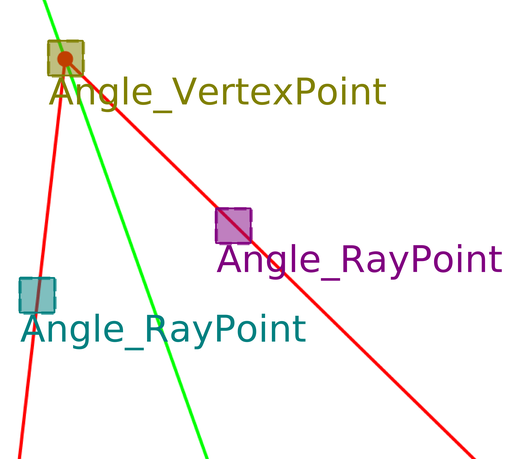
\includegraphics[width=0.3\textwidth]{img/ExampleTrainingData/02_02_secondary.png} \\
a) Input & b) Primary detection & c) Secondary detection
\end{tabular}
\caption{Sample from training data for level \textit{Beta-02}. All three parts contain the current state (red), the remaining goal (green).
Subfigure b) is a primary detection of Angle Bisector tool(purple) c) are three secondary detections: 2x angle ray point (purple, turquoise) and 1x angle vertex point(dark-yellow).}
\label{training_data_primary_02_02}
\end{figure}
Encoding clicks like in the previous subsection is not sufficient for most tools where tool parameters are position-dependent. For example, the Circle tool has two parameters: a circle center and a point on the circle. For such tools, we also have to distinguish these points. Therefore we have to add an additional target. For the Circle tool, for example, we also detect the circle center and the circle radius-point. In this thesis, we call the Circle tool detection the primary detection, and the detection intended for parameter order the secondary detection. We can see an example of primary and secondary detections in Figure \ref{training_data_primary_02_02}.
\newline \newline
Another special case is the Compass tool. We know that $\compass(A, B, C) = \compass(B, A, C)$ where $A$, $B$, and $C$ are any valid inputs from the definition of the Compass tool. This is related to the number of degrees of freedom for each tool discussed in Section \ref{degrees_of_freedom}. If a tool has this property, we can use the same object type for $A$ and $B$. This will reduce the number of object classes and also improve the problem trainability. The reason for it is that there can be multiple very similar scenes in training data that have different permutations of such points that can be switched. Then we could get to a situation where the points may be indistinguishable.


\subsection{Reducing ambiguity}
An ambiguity in a construction occurs when the next step is, for example, a random point on a given line. We would like to have every possible point on the line that does not lead to a degenerated construction in the training data. However, computing areas where points could be is extremely time-consuming. To check all degeneration criteria for a single example, we would have to check {$O(n^2)$} rules, where $n$ is the number of points in the scene. Furthermore, those areas where we cloud create a point are not even continuous, so we would have to test many points in space. On top of that, when adding multiple random points, we would have to solve whether a pair, triplet, or n-tuple of random points lead to valid construction, which would lead to exponential numbers of degeneration checks.
\newline \newline
Therefore, we reduce the ambiguity as much as we can. For example, in level \textit{Alpha-12} the goal is to find the center of a given circle. The order of the construction is:
\begin{enumerate}
  \item Angle bisector between 2 random points on the circle.
  \item Another angle bisector between 2 random points on the circle.
  \item Intersection of those angle bisectors is the circle center.
\end{enumerate}
When we want to minimize ambiguity, we need just 3 random points. It is also beneficial to fix the relative positions of these points.  We choose to fix those 3 random points to sections that correspond to points {$(1,0)$, $(-1,0)$, $(0,1)$} on the unit circle. If we do not address these ambiguities, predictions can look like in Figure \ref{mrcnn_example_01_12}, where we can see many point candidates. Having that many point candidates significantly lowers the inference accuracy.  
\newline \newline
\begin{figure}[h]
\centering
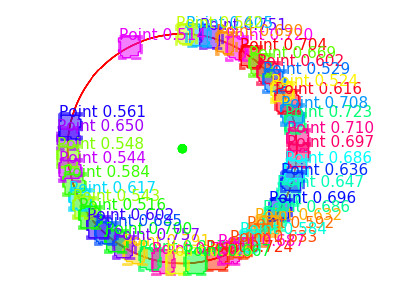
\includegraphics[width=120mm]{img/GenerationExamples/NotFixedAmbiguityCircleCenter.png}
\caption{level \texit{Alpha-12}: Find the center of a given circle. In the construction of this level, we have to create three random points on the circle, but the Mask R-CNN proposes many points due to ambiguity in training data used for training of the model. Due to the number of predicted points, we cannot use prediction like this in inference.}
\label{mrcnn_example_01_12}
\end{figure}
\section{Solving geometric constructions}
In this section we describe how we obtain actions for our Euclidea environment from the Mask {R-CNN} model.
\subsection{Mask to action}
We cannot measure the success of the model directly by its loss function. Instead, we have to measure the accuracy of level completion in the Euclidea environment. In the experiments section (see Section \ref{on_the_fly_section} and Figure \ref{on_the_fly_gen_loss}), we will see that a higher loss model can have better completion accuracy. However, we still have to monitor the loss since it should decrease during training regardless of its value.
\newline \newline
To solve Euclidea levels, we have to transform Mask {R-CNN} output to suit our environment input. The output of the model is a mask and the object type. The final layer of the Mask {R-CNN} produces a heat map, which is a probability map that gives each pixel a probability whether it is part of the mask or not. The heat map is then transformed into a mask by applying a $>0.5$ threshold to each element of the heat map. The heat map is used to create actions suitable for the environment.
\newline \newline The most straightforward actions to create are actions that correspond to the Line tool and Perpendicular Bisector tool, because these tools have a single degree of freedom. Hence we do not have to deal with  the order of the arguments. Both tools take two arguments. We take the two most probable points from the heat map that are to too close to each other. We use the same minimal distance threshold as the minimal point distance in degeneration. To find these two points, we use our version of the RANSAC algorithm \cite{Fischler81}.
\newline \newline
Now, let us describe more complicated tools. As an example, let us consider the Angle Bisector tool, which has 3 input parameters. Detection of this tool should have 4 detection outputs from Mask {R-CNN}: 1 primary and 3 secondary detections.
The primary detection is the detection of the angle bisector. Secondary detections are detections for the individual points: 
one angle vertex point and two angle ray points (see Figure \ref{training_data_primary_02_02}).
\newline \newline
To execute the tool, we have to determine the correspondence between the primary and the secondary detection.
We can obtain 3 point coordinates from the primary detection in the same way as above with the Line tool. We can also get 3 points from 3 secondary detections, each giving us one point. Each point from the primary detection corresponds to some point in the secondary detection, but these points do not exactly align. The point correspondence is then determined by minimizing distances between the primary and the secondary points (each point has to be used exactly once).
\newline \newline
\label{inferene_highest_score}
Now we can create an agent that can solve Euclidea levels. In the previous paragraph, we have described how to get an action from a single prediction.  However, Mask {R-CNN} can predict multiple actions. Mask {R-CNN} also predicts a score for each object, representing the confidence of the prediction.  For now, we can use the prediction with the highest score.  Detections with lower confidence may also be useful, and we will return to them in the next chapter.  However, multiple detections complicate the assignment of the secondary predictions. Mask {R-CNN} does not connect different detections, so we can have more secondary detections than points in the primary detection. We can still use the approach we mentioned previously, just for the assignment we no longer use each point exactly once, instead once or not at all. 
Then the agent does the following:
\label{top_score_inference}
\begin{algorithm}[h!]
\SetAlgoLined
 %\KwData{this text}
 \KwResult{Test level inference: True if level completed, False otherwise.}
 Initialize a level\;
 \While{level not complete}{
  $s \gets$ current state of the level\;
  $p \gets model.predict(s)$\;
  \If{predictions $p$ are empty}{
   \Return False\;
   }
  $a \gets$ action from $p$ with highest score\;
  execute $a$
 }
 \Return True\;
 
\caption{Inference: Top score prediction}
\end{algorithm}

In Table \ref{EuclideaExample-Network}, we can see an example solution of the geometric problem solved using top score predictions.

\subsection{Incomplete detections}
There are instances of levels with incomplete detections. A detection is incomplete if there are not enough points in the primary or the secondary detection. If there are not enough primary points, we cannot determine any action. For secondary points, we can determine as many points as possible, and then the rest of the points can be randomly assigned. Applying a random assignment is frequently used in inference, mostly for the Circle tool. Many constructions use a sequence of $\circletool(A, B)$ followed by $\circletool(B, A)$ to obtain equilateral triangle, perpendicular bisector, midpoint of a segment, 60$^{\circ}$ degree angle, etc. During inference of this situation based on data from the first detection, we have to construct either $\circletool(A, B)$ or $\circletool(B, A)$ and the second detection has to construct the other circle. When we go through Euclidea levels while creating the training data, we have to choose which step we do first.
Furthermore, because we generate level instances randomly, there can be multiple similar level instances during training that choose different moves, i.e.~there are two samples in training data that have the same primary detections but different secondary detections. During training, those secondary detections may cancel each other out resulting in the primary detection without the secondary one. However, as mentioned above, we can use any action defined by the detected primary actions. This effect occurs mostly for the Circle tool, but it can occur for other tools as well.
\subsection{Opposite corner detection}
Some detections may miss click coordinates even in the primary detections. However, the prediction of a bounding box can still be predicted correctly. If a tool has 2 arguments, we can find another point in this situation with point reflection. We reflect the detected point with the center of symmetry in the center of the bounding box. The bounding box for the training data is a minimal bounding box containing the mask in the training data. Hence when we expect the output to have 2 click coordinates, one point is in a corner, and the other is in the opposite corner of the bounding box.

\section{Other models}
Before we experimented with Mask {R-CNN}, we tried models that predict action click coordinates straight from images. The output of the model were coordinates, not a mask. We used a convolutional network with few densely connected layers and two output layers: a softmax layer that predicted the tool index and a layer with 6 outputs representing x and y coordinates of 3 points. The activation function for the layer predicting coordinates was the sigmoid activation multiplied by the window size (size of the input image). Hence all predictions were valid coordinates within the image. However, this model had problems even on simple levels like \textit{Alpha-01}. It was able to do the 1st step of \textit{Alpha-01}, but then it was never able to predict the second step correctly. Although the model was able to detect points in \texit{Alpha-01}, it could not detect already constructed lines, and thus the model was trying to construct one line repeatedly. The model had even worse results on levels that use position-dependent tools. It also produce only one output compared to Mask {R-CNN}, where we can use multiple outputs as potential moves.


\begin{longtable}{p{0.48\textwidth}p{0.48\textwidth}}

\subfloat{\includegraphics[width = 2.5 in]{img/Equilateral_example/input_image0.png}} &
\subfloat{\includegraphics[width = 2.5 in]{img/Equilateral_example/output_image0.png}}\\

 a) Initial configuration & b) Construction step: 1. Based on the prediction a circle will be constructed.\\
 %and first prediction & and second prediction \\

\subfloat{\includegraphics[width = 2.5 in]{img/Equilateral_example/output_image1.png}} &
\subfloat{\includegraphics[width = 2.5 in]{img/Equilateral_example/output_image2.png}}\\

c) Construction step: 2. Based on the prediction a circle with a different center then in last step will be constructed.   & d) Construction step: 3. Based on the prediction a line will be constructed. \\[5cm]
%and third prediction & and fourth prediction \\

\subfloat{\includegraphics[width = 2.5 in]{img/Equilateral_example/output_image3.png}}&
\subfloat{\includegraphics[width = 2.5 in]{img/Equilateral_example/input_image4.png}}\\
e) Construction step: 4. Based on the prediction a line will be constructed. &
f) Construction step: 5 - level finished &\\
%f) construction step: 5 - level finished \\
%and sixth prediction &  \\


\caption{Sequence of construction steps with predictions for the Euclidea level \textbf{Alpha-01} Equilateral Triangle. The first state is the level definition consisting of the initial configuration (red) and the remaining goal (green). In each step, our approach predicts the usage of one tool towards constructing the goal.}
\label{EuclideaExample-Network}
\end{longtable}

\chapter{Solving unseen geometric constructions}
\label{chapter_unseen_levels}
We have already mentioned, there are multiple predictions in Mask {R-CNN} models (see Section \ref{inferene_highest_score}). In this chapter, we further examine those predictions. To do so, we create a program for the exploration of hypotheses given by multiple models. Then we introduce the hypothesis tree search for solving unseen levels. Lastly, we analyze the inference of unseen levels with the leave-one-out method.
\section{Hypotheses generated by Mask {R-CNN}}
Each primary detection by the Mask {R-CNN} model described in Chapter \ref{mrcnn_chapter} can be transformed into an action. We denote each action, its arguments and results as ``hypothesis''. The result of an action contains the reward and output geometric primitive constructed during the action execution. The reward indicates whether the output primitive is a part of the goal or not. If an action constructs part of the goal, the reward is equal to $1/n$, where $n$ is the number of primitives in the goal, otherwise, it is equal to zero. In Table \ref{hypothesis_explorer_detail} in Sub-figure d) we can see a hypothesis that successfully finished one of the four goals and hence it has a reward equal to $0.25$.  We  can extract multiple actions from the Mask R-CNN model outputs and then transform them into multiple hypotheses. 
\newline \newline
When we obtain hypotheses from the Mask {R-CNN}, we can explore the construction space defined by those hypotheses. Furthermore, we can also use hypotheses from multiple models trained for different tasks. However, Mask {R-CNN} scores across hypotheses from different models are not well calibrated. For exploration purposes, we developed an interactive program where the user can choose multiple trained models and levels for inference, and then run inference where the user can choose which hypothesis should be used at a given time. In Figure \ref{hypothesis_explorer} we can see a screenshot from the program followed with hypotheses details in Table \ref{hypothesis_explorer_detail}. Hypothesis visualization is based on our Euclidea visualization (see Section \ref{euclidea_vizualization}) with the addition of the hypothesis result object to the blue channel. The program can get hypotheses from any model, but in this thesis, we prepared models trained on the first 6 Euclidea level packs:
\begin{itemize}
\item 68 ``level'' models (one for each level). 
\item 6 ``level-pack'' models (one for each level pack).
\item 1 ``all'' model (for level packs Alpha - Zeta).
\end{itemize}

\begin{figure}[h!]
\centering
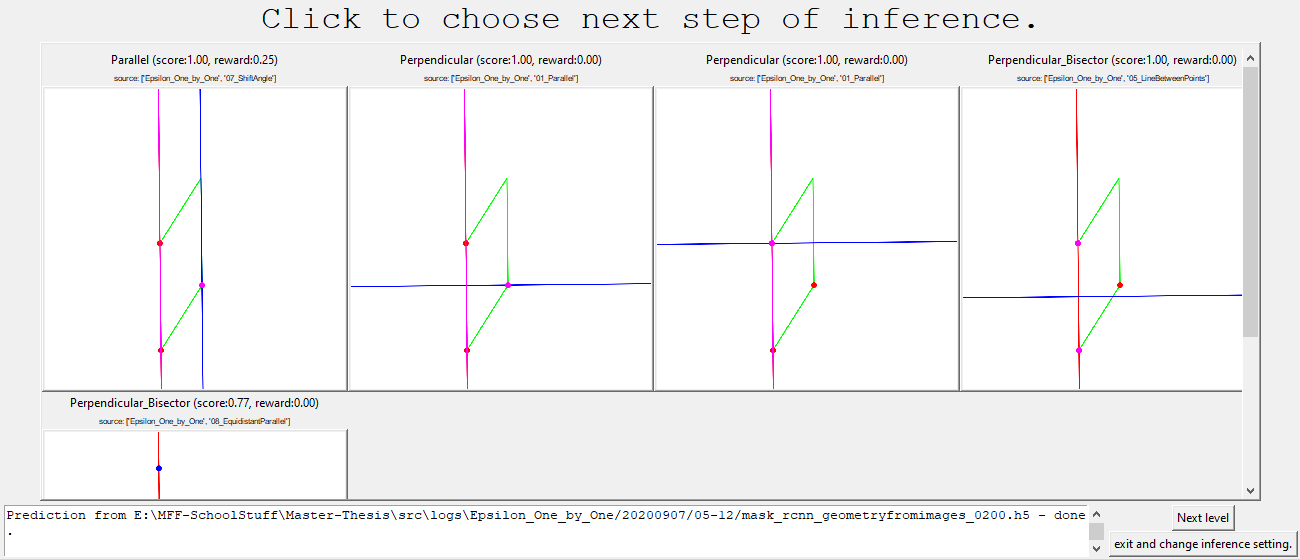
\includegraphics[width=140mm]{img/hypothesis_explorer/explorer.png}
\caption{Screenshot of our hypothesis explorer program. Construction of the level \textit{Epsilon 03}, Parallelogram given by 3 points. To solve this level, we have all level-specific models for Epsilon, with the exception of the model for \textit{Epsilon 03}. In this step of construction, we have 5 different hypotheses given by 4 models. Other models either do not give any hypotheses or give hypotheses that can be grouped with other hypothesis (see Section \ref{reducing_hypotheses}), we consider only a single hypothesis per group. In the program, the user chooses manually which hypothesis should be constructed. Details of each hypothesis are in Table \ref{hypothesis_explorer_detail} }
\label{hypothesis_explorer}
\end{figure}

\begin{longtable}{m{0.5\textwidth}m{0.5\textwidth}}
         \begin{subfigure}
         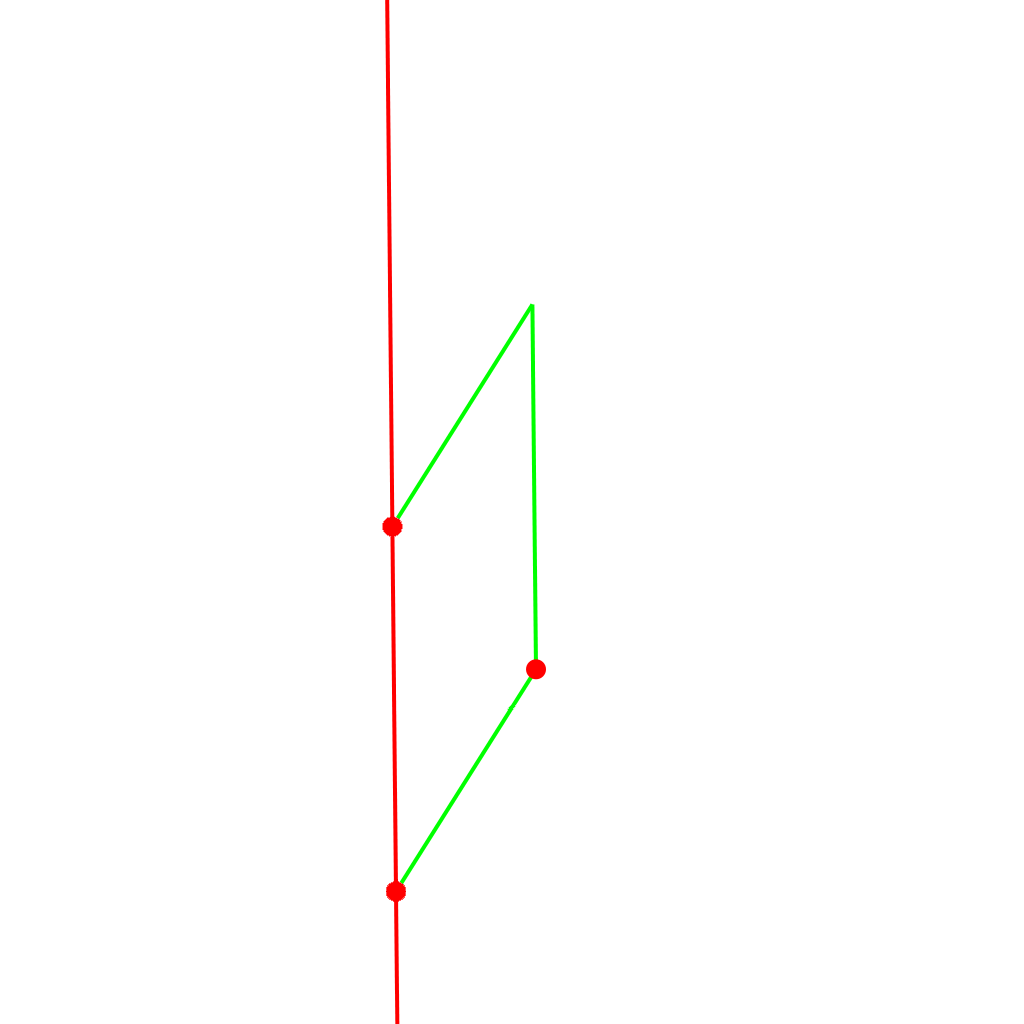
\includegraphics[width=70mm]{img/hypothesis_explorer/input.png}
         \label{xx}
         \end{subfigure}
         &
         \begin{subfigure}
         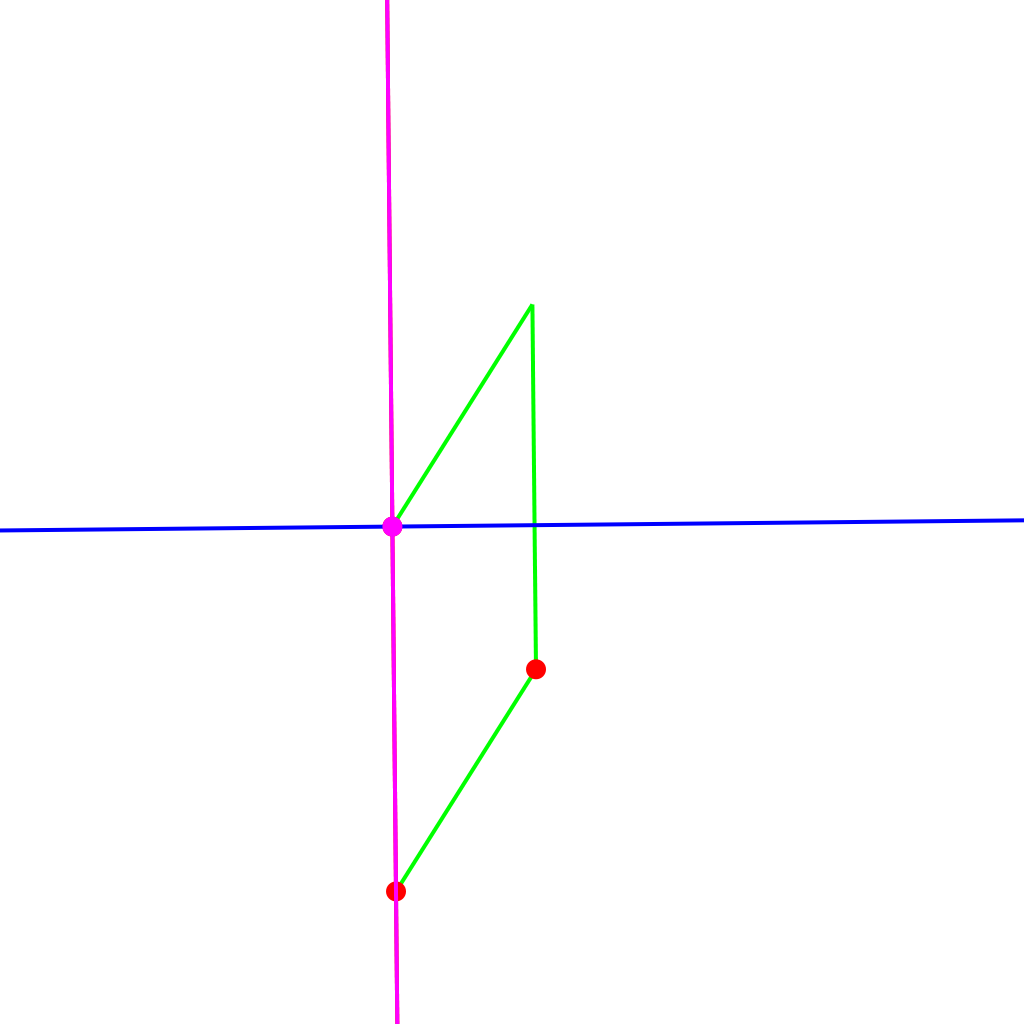
\includegraphics[width=70mm]{img/hypothesis_explorer/source_01_score_0.999_Perp.png}
         \label{xx}
         \end{subfigure}
         \\
         a) The Current state without any hypothesis, Input for the Mask {R-CNN} models. &
         b) source: Epsilon 01, score: 0.99, tool: Perpendicular, reward: 0.0 \\
         \begin{subfigure}
         \includegraphics[width=70mm]{img/hypothesis_explorer/source_05_score_0.996_PerpBisector.png}
         \end{subfigure}
         &
         \begin{subfigure}
         \includegraphics[width=70mm]{img/hypothesis_explorer/source_07_score_0.999_Parallel.png}
         \end{subfigure}
         \\
          c) source: Epsilon 05, score: 0.99, tool: Perpendicular Bisector, reward: 0.0 &
         d) source: Epsilon 07, score: 0.99, tool: Parallel line, reward: 0.25\\
         \begin{subfigure}
         \includegraphics[width=70mm]{img/hypothesis_explorer/source_08_score_0.77_PerpBisector.png}
         \end{subfigure}
         &
         \begin{subfigure}
         \includegraphics[width=70mm]{img/hypothesis_explorer/source_01_score_0.999_Perpl.png}
         \end{subfigure}
         \\
         e) source: Epsilon 08, score 0.77, tool: Perpendicular Bisector, reward: 0.0 &
         f) source: Epsilon 01, score: 0.99, tool: Perpendicular, reward: 0.0 
         \\
\caption{Five different hypotheses for solving the level \textit{Epsilon 03}. This table is a detail for Figure \ref{hypothesis_explorer}. Thus each hypothesis corresponds to its miniature in Figure \ref{hypothesis_explorer}. Each figure contains the current state (red), remaining goal (green), hypothesis produced by Mask R-CNN (blue), and highlighted arguments of the tool (purple). We can see that hypothesis d) has a reward equal to $0.25$. Hence d) is a correct step that should be picked in this step.}
\label{hypothesis_explorer_detail}
\end{longtable}

\section{Inference with tree search}
\label{hypotheses_tree_search}
In the previous section, we described how to get hypotheses from multiple Mask {R-CNN} models. Now we will search for the target construction within these hypotheses. To compare the results of the hypothesis tree search with the exhaustive tree search from Chapter \ref{chapter_exhaustive_search}, we use iterative deepening. The tree search has to build an input image and run predictions of all Mask {R-CNN} models in each node, which significantly increases the time spent on one node. However, the hypothesis tree search should have a significantly lower branching factor.

\section{Reducing the number of hypotheses}
\label{reducing_hypotheses}
Hypotheses produced by different models increase the branching factor and thus also the search time. In order to speed up the tree search, we group similar hypotheses and explore only one of them. We consider two hypotheses to be similar if they have the same output geometric primitive. Note that they can have different arguments, including different tools.

\section{Cheat moves}
In Euclidea, a goal cannot be finished by simply drawing a similar line or circle (see Section \ref{about_euclidea}). We denote those as cheat moves. However, a hypothesis given by the models may suggest drawing a cheat move. We can recognize some hypothesis of a cheat move by coordinates of its arguments. One of its arguments is a point in space without any geometric primitive nearby. Note that with the mentioned approach, we cannot find every cheat move. Some levels aim to find a specific point on the line or circle, which can be guessed instead of constructed. Cheat move hypotheses can be removed as they do not lead to the goal. However, when all necessary points are constructed further in construction, this cheat move prediction becomes a legitimate move.

\section{Leave-one-out evaluation}
\label{leave_one_out_method}
We use the ``leave-one-out'' method to evaluate performance on unseen levels. For our purposes the method inputs are levels with corresponding level specific models. To evaluate accuracy of a level we use all other models, e.g.~models that were not trained for this level. We can also apply this on whole level pack models. Note that we should avoid a situation where 2 different models are trained for the same task, for example we should not have models for \textit{Alpha 01} level and Alpha level pack, since both models are trained for \textit{Alpha 01}. For the inference we use the hypothesis tree search (see Section \ref{hypotheses_tree_search}).
Note that due to score miss calibration, the top score detection (see Section \ref{top_score_inference}) approach cannot be used when we have multiple models. The accuracy of the leave-one-out set-up is reported in the experimental Section \ref{eval_of_unseen_levels}.

\section{Connections between levels}
\label{connections}
When evaluating a level using leave-one-one method, we might use hypotheses only from a fraction of level specific models. We denote that level $X$ is ``connected'' to level $Y$, when a model trained for $Y$ contributes to a successful construction with any hypothesis during the inference for level $X$. Note that relation ``connected'' is not reflexive, e.g.~ when $X$ is connected to $Y$, then $Y$ is not necessary connected to $X$. Since we run hypothesis tree search during the leave-one-out evaluation, we obtain connections in following way: If the search is successful, we collect models that contributed to the solution in the final backtracking of the search.



\chapter{Experiments}
\label{experiment_chapter}
This chapter describes the components of our model and how they affect model performance on Euclidea levels \ref{design_choices}. Furthermore, we analyze the performance of the best model \ref{supervised_evaluation} and the leave-one-out method performance on unseen levels \ref{eval_of_unseen_levels}. Then we show example solutions of levels \ref{example_of_level}.
\section{Algorithm design choices}
\label{design_choices}
This section describes the different components of our model and the training set-up. In each subsection, we describe a new component of our approach that improves accuracy. We start with our initial model that had only a low accuracy on the Alpha level pack and then add the different components that we have designed to improve the accuracy of the model.
\newline \newline
Levels can be solved using different constructions. Some constructions can be more trainable than others, e.g.~ a model trained for construction $A$ of level $X$ might have higher accuracy than a model trained for construction $Y$ of level $X$. Note that construction $A$ and $B$ can be completely different constructions but also can differ only in the permutation of construction steps. Also, the probability of degenerated scenes varies across different constructions. In practice, this probability should be low enough so as not to slow down the data generation. Therefore, before training a new level pack, we first ensure that all its levels are trainable by level-specific models. 
\newline \newline
%\subsection{Reducing inference complexity}
Some models have difficulty deciding which tool should be used at a given state of the construction. To make it less complicated, we are using hints. To generate random instances of a level, we have to compute its construction as well (see Section \ref{degen_criteria}). Since the models aim to mimic this construction, we provide them with hints which tool should be used at a given time. The hints are not included in the Mask {R-CNN} input but instead, we consider only detections with a tool index corresponding to the hint. We use hints to compare accuracies with and without hints. Hints are used for our initial models that were not able to solve the most manageable levels.

\subsection{Detection of points and intersections}
\label{no_point_detection}
In our version of Euclidea, we are limited in using tools with point arguments. Let us consider example construction: Construction of the midpoint of a given segment $AB$. We already constructed two circles, $\circletool(A, B)$ and $\circletool(B, A)$. The last step is to make a line given by two intersections of circles.  However, we cannot do so because intersections are not marked as points. Instead, we have to use the Point tool on each intersection, and only then can we create the line. To draw the line without the need to mark the points, we use the automatic point detection. It is realized when we execute a tool. The environment returns whether the tool was executed successfully or not. If not, we can use the Point tool on each argument to mark these points. This change allows us to reduce the usage of the Point tool only if the level has a goal to find a specific point: center of the triangle etc. 
\newline \newline
In Figure \ref{no_point_detection_img} we can see a potential problem if we do not use the automatic point detection. Based on the figure detection, we would be creating all points since they have a high Mask {R-CNN} score and we would not use the Circle tool.
\begin{figure}[t]
\centering
\includegraphics[width=100mm]{img/NO_POINT_DETECTION.png}
\caption{Example of the detection for level \textit{Alpha-10}, the goal of this level is to construct an incircle of a given square. The figure shows the current state of the construction (red), the remaining goal (green) and multiple detections of the Point Tool and Circle tool. The figure shows a potential problem if we do not use the automatic point detection (see Section \ref{no_point_detection}). If we do not use the automatic point detection, we have to detect usages of the Point tool as well. Then the network might prefer creating many points instead of using other tools.}
\label{no_point_detection_img}
\end{figure}

\begin{table}[t]
    \centering
    \begin{tabular}{| p{0.25\textwidth} | p{0.13\textwidth} | p{0.13\textwidth} | p{0.13\textwidth} | p{0.13\textwidth} |}%
    \hline
\multirow{2}{*}{\bfseries{Alpha levels}} &
\multicolumn{2}{m{0.3\textwidth}|}{\bfseries{without automatic point detection}} & \multicolumn{2}{m{0.3\textwidth}|}{\bfseries{automatic point detection}}
    \\
     & \bfseries Hints & \bfseries No hints & \bfseries Hints & \bfseries No hints
    \\\hline
    \csvreader[head to column names,late after line=\\, before filter=\ifthenelse{\equal{\csvcoli}{Accuracy}}{\csvfilterreject}{\csvfilteraccept}]{../img/tables/no_point_detection.csv}{}% use head of csv as column names
    {\level  & \PreviousHints & \Previous & \NoPointHints & \NoPoint}
    \hline
    \csvreader[head to column names, before filter=\ifthenelse{\equal{\csvcoli}{Accuracy}}{\csvfilteraccept}{\csvfilterreject}]{../img/tables/no_point_detection.csv}{}% use head of csv as column names
    {\bfseries{Average}  & \bfseries{\PreviousHints} & \bfseries{\Previous} & \bfseries{\NoPointHints} & \bfseries{\NoPoint}}
    \\\hline
    
    \end{tabular}
    \caption{Accuracy of Alpha levels during inference for the model with and without automatic point detection, evaluation on 500 instances for each level with and without hints. Note that some accuracies with hints can be slightly higher than without hints. Different permutations of construction steps can change the predictions of the model. When we use hints, we choose a prediction with the highest score that matches a hint, but there can be a higher score that does not match the hint.}
    \label{no_point_detection_table}
\end{table}

From Table \ref{no_point_detection_table} it is clear that automatic point detection improves the accuracy of every level. We can also see that automatic point detection no longer needs hints, as there is little difference between hint and no hints accuracy.
\subsection{History channel, more data on the input}
\label{history_channel}
Models generally have a problem to determine the exact step of the construction. We can observe that a single detection contains predictions of actions that correspond to actions used in later stages of the construction. In most cases, actions that are supposed to be used later have a lower Mask {R-CNN} score, but when they have a higher score, then we cannot solve the level by choosing only the top scoring hypothesis (see Section \ref{top_score_inference}). To avoid these situations, we add a history channel to the training data. With the current state in the first channel, the goal in the second channel, we add the previous state to the third channel. Furthermore, we can add a state before 2 steps to the fourth channel, a state before 3 steps to the fifth, and so on. However, we use only one history channel because we use the pre-trained Mask {R-CNN} model, and increasing the number of channels over 3 (over 1 history channel) we would have to train the whole Mask {R-CNN} model, including its backbone.

\begin{table}[th!]
    
    \begin{tabular}{| p{0.25\textwidth} | p{0.13\textwidth} | p{0.1\textwidth} |}%
    \hline
    \bfseries Alpha levels & \bfseries Without history & \bfseries With history
    \\\hline
    \csvreader[head to column names,late after line=\\,before filter=\ifthenelse{\equal{\csvcoli}{Accuracy}}{\csvfilterreject}{\csvfilteraccept}]{../img/tables/history_channel.csv}{}% use head of csv as column names
    {\level & \withouthistory & \withhistory}
    \hline
    \csvreader[head to column names, before filter=\ifthenelse{\equal{\csvcoli}{Accuracy}}{\csvfilteraccept}{\csvfilterreject}]{../img/tables/history_channel.csv}{}% use head of csv as column names
    {\bfseries{Average} & \bfseries{\withouthistory} & \bfseries{\withhistory}}
    \\\hline
    \end{tabular}
    \begin{tabular}{|p{0.25\textwidth} | p{0.1\textwidth} |}
         \hline
    \bfseries Beta levels & \bfseries With history
    \\ \hline
    \csvreader[head to column names,late after line=\\, before filter=\ifthenelse{\equal{\csvcoli}{Accuracy}}{\csvfilterreject}{\csvfilteraccept}]{../img/tables/history_channel.csv}{}% use head of csv as column names
    {\betalevel & \betawithhistory}
    \hline
    \csvreader[head to column names, before filter=\ifthenelse{\equal{\csvcoli}{Accuracy}}{\csvfilteraccept}{\csvfilterreject}]{../img/tables/history_channel.csv}{}% use head of csv as column names
    {\bfseries{Average} & \bfseries{\betawithhistory}}
    \\\hline
    \end{tabular}
    \caption{Accuracy of levels for the model with and without history (see Section \ref{history_channel}), evaluation on 500 instances for each level, for Alpha pack on the left and Beta pack on the right. Note that for Beta there is inference only with history. Model without history was not working on Beta at all. Models are based on the model with automatic point detection (see Section \ref{no_point_detection}).}
    \label{history_channel_table}
\end{table}

In Table \ref{history_channel_table} we can see an improvement of accuracy on the Alpha levels. Moreover, models with history were the first models that learned Beta levels with reasonable accuracy.
\newpage
\subsection{Stages of Mask {R-CNN}}
\label{stages_of_mercnn}
\begin{table}[h!]
    \centering
    \begin{tabular}{| p{0.25\textwidth} | p{0.13\textwidth} | p{0.08\textwidth} |}
    \hline
    \bfseries Beta levels & \bfseries Without 4+ & \bfseries With 4+ 
    \\\hline
    \csvreader[head to column names,late after line=\\, before filter=\ifthenelse{\equal{\csvcoli}{Accuracy}}{\csvfilterreject}{\csvfilteraccept}]{../img/tables/4plustraining.csv}{}% use head of csv as column names
    {\level & \previous & \fourplus }
    \hline
    \csvreader[head to column names, before filter=\ifthenelse{\equal{\csvcoli}{Accuracy}}{\csvfilteraccept}{\csvfilterreject}]{../img/tables/4plustraining.csv}{}% use head of csv as column names
    { \bfseries{Average} & \bfseries{\previous} & \bfseries{\fourplus} }
    \\\hline
    
    \end{tabular}
    \caption{Accuracy of levels during inference for models trained with the following setups. \textbf{Without 4+}: first 120 epochs training of head layers, then 80 epochs training the whole network. \textbf{With 4+}: first 60 epochs training of head layers, then 60 epochs of 4+ layers and then 80 epochs training the whole network. Both models have a history (see Section \ref{history_channel}), 500 instances of each level. Note that model without 4+ is the same model for Beta mentioned in Section \ref{history_channel_table}.}
    \label{four_plus_table}
\end{table}

Training of the Mask {R-CNN} is often divided into several stages. Each stage can have different training parameters. For training purposes, we have a stage with head layers, which are layers that compute masks from features detected in the backbone, and a stage with the backbone. The implementation of Mask {R-CNN} we use \cite{matterport_maskrcnn_2017} divides the backbone into multiple stages. It divides the backbone into 5 stages and allows to train only stages 3 and up, 4 and 5. We denote ``4+'' as training of the 4th and 5th stage of backbone and all head layers. Until now, we were using the following training setup: First, we train only head layers of Mask {R-CNN} and then we train the whole network. In Table \ref{four_plus_table} we can see the difference in accuracy if we include 4+ training, which shows that 4+ training improves accuracy on the beta level significantly. In Figure \ref{four_plus_losses} we can also see that models with 4+ training have a smoother loss. Spikes in epoch 60 and 120 are caused by enabling more layers to be trainable e.g.~first 60 epoch, we train only the head layer, and then we start 4+ as well. From epoch 120 we train the whole network.

\begin{figure}[h]
\centering
%models: logs/redoing_alpha/alpha_again_minimask ; logs/redoing_alpha/alpha_4+_included
\includegraphics[width=140mm]{img/4+_losses.png}
\caption{Comparison of loss functions for training with and without 4+ training set-up (see Section \ref{stages_of_mercnn}). \textbf{Alpha without 4+} : epochs 0-120 training only heads, epochs 120-200 training the whole network. \textbf{Alpha with 4+} : epochs 0-60 training only heads, epochs 60-120 training only layers 4+ (i.e. backbone stages 4, 5 and the heads) and epochs 120-200 training the whole network. The loss for training with 4+ layers (blue) is much smoother and is less spiky than without 4+ (orange). }
\label{four_plus_losses}
\end{figure}

\subsection{Multiple solutions problem}

\begin{figure}[h!]
\centering
\begin{tabular}{ m{5cm} m{5cm}}
    \begin{subfigure}
    \includegraphics[width=47mm]{img/Gamma_gen_problem.png}
    \caption{}
    \label{gamma_close_dual_constr_main}
    \end{subfigure}
    &
    \begin{subfigure}
    \fbox{\includegraphics[width=47mm]{img/Gamma_gen_probem_detail.png}}
    \caption{detail of the orange area of Figure \ref{gamma_close_dual_constr_main}}
    \label{gamma_close_dual_constr_detail}
    \end{subfigure}
    \\
\end{tabular}
    
   
\caption{The degenerated instance of the level \text{Gamma-04}, the first step of the construction done. The goal is to find $X \in p, Y \in q$ such that $|MX| = |MY|$. Both solutions are very close to each other, and it is hard to recognize which solution we are supposed to construct. See detail in Figure \ref{gamma_close_dual_constr_detail}. Thus constructions are close as well. Hence the instance is degenerated. The degenerated configurations should not be in the training data nor in testing data because they are unsolvable based on image data.}
\label{gamma_close_dual_constr}
\end{figure}
To improve our generation process, we added the fourth degeneration rule: Intersections of geometric primitives can not be too close to the construction points (see Section \ref{degen_criteria}). The fourth rule was not applied to the data generation process while training and running inference for models in the sections above. Levels from Alpha and Beta packs are rarely considered as degenerated by the fourth rule. However, levels in the Gamma pack and above are. Some levels in Gamma are untrainable. Examples of these  are \textit{Gamma-04} and \textit{Gamma-05}. Around $27\%$ of \textit{Gamma-04} instances are considered as degenerated by the fourth rule while considered as valid by rules 1.~-3.~, in Figure \ref{gamma_close_dual_constr} we can see an example of this. This change allowed us to train Gamma and Delta levels. In Table \ref{new_gen_gamma_delta} we can see results if we add the fourth rule to the data generation. Level \textit{Delta-06}, construction of $\sqrt{2}$, has accuracy equal to $0$, because it is very similar to the \textit{Delta-07}, construction of $\sqrt{3}$, and models tend to prefer only one of these two levels. 


\begin{table}[h]
    \begin{tabular}{| p{0.28\textwidth} | p{0.15\textwidth} |}
    \hline
    \bfseries Gamma levels & \bfseries Accuracy 
    \\\hline
    \csvreader[head to column names,late after line=\\, before filter=\ifthenelse{\equal{\csvcoli}{Accuracy}}{\csvfilterreject}{
    \ifthenelse{\equal{\csvcoli}{}}{\csvfilterreject}{\csvfilteraccept}}]{../img/tables/gamma_delta_newgen.csv}{}% use head of csv as column names
    {\gammalevel & \gammaacc}
    \hline
    \csvreader[head to column names,late after line=\\, before filter=\ifthenelse{\equal{\csvcoli}{Accuracy}}{\csvfilteraccept}{\csvfilterreject}]{../img/tables/gamma_delta_newgen.csv}{}% use head of csv as column names
    { \bfseries{Average} & \bfseries{\gammaacc}}
    \hline
    
    \end{tabular} 
    \begin{tabular}{|p{0.28\textwidth} | p{0.15\textwidth} |}
        \hline
         \bfseries Delta levels & \bfseries Accuracy
         \\\hline
         \csvreader[head to column names,late after line=\\, before filter=\ifthenelse{\equal{\csvcoli}{Accuracy}}{\csvfilterreject}{\csvfilteraccept}]{../img/tables/gamma_delta_newgen.csv}{}% use head of csv as column names
        { \deltalevel & \deltaacc}
        \hline
        \csvreader[head to column names,late after line=\\, before filter=\ifthenelse{\equal{\csvcoli}{Accuracy}}{\csvfilteraccept}{\csvfilterreject}]{../img/tables/gamma_delta_newgen.csv}{}% use head of csv as column names
        { \bfseries{Average} & \bfseries{\deltaacc} }
        \hline
    \end{tabular}
    \caption{Accuracy of models for Gamma and Delta level packs for a new data generation. We include new degeneration rule: Intersections of geometric primitives can not be too close to the construction points (see (see Section \ref{degen_criteria}). Evaluation for Gamma level peck on the left and for the Delta level pack on the right. Note that the model with the fourth rule applied was the first model that was successfully able to solve Gamma and Delta level packs.}
    \label{new_gen_gamma_delta}
\end{table}
\subsection{On-the-fly generation}
\label{on_the_fly_section}
Until now, we were using pre-generated training data that had to be stored in memory. Pre-generated levels have to be in memory. Thus there is a limit to the size of the training data. The models described above contained 100 000 finished constructions of levels, the average length of construction is around 5 steps, thus 500 000 training examples had to be stored. To further increase the number of samples, we use generation on-the-fly, so each sample is seen only once during the training. Keep in mind that history, degeneration checks, and multi-thread training have to be adjusted as well. In Figure \ref{on_the_fly_gen_loss}
we can make a comparison of losses for models using pre-generated and on-the-fly generation. The loss of the model with on-the-fly generation decreases at a lower rate. However, the loss function is smoother, and the model achieves better accuracy during inference. The accuracy is equal to $0.991$, compared to $0.735$ accuracy of the model with a pre-generated dataset. Although a model with on-the-fly generation has a higher loss value, it generalizes better due to the variety of the training data, e.g.~the model with pre-generated data is prone to over-fitting.
\begin{figure}[h]
\centering
\includegraphics[width=\textwidth]{img/on-the-fly-gen.png}
\caption{Loss of models that uses 500k pre-generated training examples (Delta pre-generated) and 3.2M training examples generated on-the-fly (Delta on-the-fly).  Both networks were trained in the following setup: epochs 0-60 training only heads, epochs 60-120 training only layers 4+ (i.e. backbone stages 4, 5 and the heads) and epochs 120-200 training the whole network. Note that pre-generated training data are forwarded in the network with in a random order, but samples generated on-the-fly are fed to the network in the order they were created.}
\label{on_the_fly_gen_loss}
\end{figure}
\section{Evaluation of supervised learning approach}
\label{supervised_evaluation}
With components described in the previous Section \ref{design_choices}, we can train models that can solve entire packs or even multiple packs at once. We evaluate models on the first six level packs (Alpha, Beta, Gamma, Delta, Epsilon, Zeta). All those packs are prepared for data generation, and thus to training. 
\newline \newline
We trained a model for each level (68) for the first 6 level packs of Euclidea. Each model is trained for 200 epochs. Each epoch consists of 16~000 training samples, e.g.~1~000 training steps of batches of size 16. The model generates data on-the-fly (see Section \ref{on_the_fly_section}). Hence $3.2M$ training samples are seen during the training. In the first 120 epochs, we train only head layers, then 60 epochs of 4+ layers and the last 60 epochs train the whole network (see Section \ref{stages_of_mercnn}). Initial weights of the model are weights from the COCO model, which is part of Matterport \cite{matterport_maskrcnn_2017}. This model has an average $97.7\%$ accuracy, which has been evaluated on 500 instances for each level in Alpha to Zeta packs. Results are summarized in Table \ref{final_model_results}.
\newline \newline
We also trained single model for each level pack. Models for level packs are trained in the same way, and the only difference is the number of epochs. Level pack models are trained for 260 epochs: 120 heads, 60 epochs of 4+ and 80 epochs of the whole network. Level pack models have the following accuracies reported in Table \ref{final_model_results}.
\newline \newline
Finally, we trained a single model for all levels. The training setup of this model is the same as for individual models and level pack models. The only difference is the number of epochs. The model was trained for 400 epochs ($6.4M$ training samples): 200 heads, 100 of 4+ and 100 of the whole network. This model has an average $91.8\%$ accuracy and the hypothesis tree search accuracy of $92.1\%$. Accuracies for each level are in Appendix \ref{all_model_tree_search}).
\newline \newline
\begin{table}[h]
\begin{tabular}{l| l l l l l l}
Model / Level Pack & Alpha & Beta & Gamma & Delta & Epsilon & Zeta
 \\ \hline
 one model per level & $98.7\%$ & $98.6\%$ & $97.4\%$ & $99.3\%$ & $96.3\%$ & $96.0\%$\\
 one model per pack & $96.1\%$& $96.2\%$ & $97.8\%$& $99.1\%$ & $92.8\%$ & $95.7\%$ \\
 one model for all levels & $90.0\%$ & $94.4\%$ & $89.4\%$ & $96.9\%$ & $88.6\%$ & $91.5\%$ \\
 \end{tabular}
 \caption{Final results of models for all levels, level packs and individual models. Each column represents the average accuracy of the model(s) on all levels (500 instances for each level) of a respective pack. \textbf{Individual models}: One model for each of 68 levels, accuracy is measured only for a model on a corresponding level. \textbf{level pack models}: One model for each of 6 level packs. Inference of the pack measured for a model trained for a respective pack. \textbf{all level model}: One model is used for all levels.}
 \label{final_model_results}
\end{table}

\section{Evaluation of supervised learning on unseen problems
}
\label{eval_of_unseen_levels}
To evaluate a model's performance on unseen levels, we use the leave-one-out method with the hypothesis tree search (see Sections \ref{hypotheses_tree_search} and \ref{leave_one_out_method}).  We use models for all levels and all level packs from the previous chapter. The results are shown in Figures \ref{leave_one_out_levels} and \ref{leave_one_out_packs} we can see results of the leave-one-out evaluation of hypothesis tree search. Some levels can be solved this way, but others cannot. To solve an unseen level, we have to have parts of the construction in models we have seen in training, e.g.~ the first part of the construction can be done with a model X and the second part with a model Y.
\begin{table}[ht]
    \centering
    \begin{tabular}{ p{0.30\textwidth}  p{0.15\textwidth}  p{0.45\textwidth}}
    %\hline
    \bfseries Level & \bfseries Accuracy & \bfseries Connections
    % \hline
    \end{tabular}
    \vspace*{2mm}
    \textbf{Alpha}
    \begin{tabular}{ p{0.30\textwidth}  p{0.15\textwidth} p{0.45\textwidth}}
    \hline
    %\bfseries Level & \bfseries Accuracy & \bfseries Connections
    \csvreader[head to column names,separator=semicolon
    ]{../img/tables/leave_one_out_levels_alpha.csv}{}% use head of csv as 
    {\\[0.05cm]\level & \accuracy & \connections}
    \end{tabular}
    \textbf{Beta}
    \begin{tabular}{ p{0.30\textwidth}  p{0.15\textwidth}  p{0.45\textwidth}}
    \hline
    \csvreader[head to column names,separator=semicolon ]{../img/tables/leave_one_out_levels_beta.csv}{}% use head of csv as 
    {\\[0.05cm]\level & \accuracy & \connections}
    %\hline
    \end{tabular}
    \textbf{Gamma}
    \begin{tabular}{ p{0.30\textwidth}  p{0.15\textwidth}  p{0.45\textwidth}}
    \hline
    \csvreader[head to column names,separator=semicolon ]{../img/tables/leave_one_out_levels_gamma.csv}{}% use head of csv as 
    {\\[0.05cm]\level & \accuracy & \connections}
    %\hline
    \end{tabular}
    \textbf{Epsilon}
    \begin{tabular}{ p{0.30\textwidth}  p{0.15\textwidth} 
    p{0.45\textwidth}}
    \hline
    \csvreader[head to column names,separator=semicolon ]{../img/tables/leave_one_out_levels_epsilon.csv}{}% use head of csv as 
    {\\[0.05cm]\level & \accuracy & \connections}
    %\hline
    \end{tabular}
    \textbf{Zeta}
    \begin{tabular}{p{0.30\textwidth}  p{0.15\textwidth}  p{0.45\textwidth}}
    \hline
    \csvreader[head to column names,separator=semicolon ]{../img/tables/leave_one_out_levels_zeta.csv}{}% use head of csv as 
    {\\[0.05cm]\level & \accuracy & \connections}
    \\
    \end{tabular}
    
    
   \caption{Leave-one-out evaluation of hypothesis tree search for each level pack. Model for \textbf{each level} within a pack are inputs for the method, e.g.~accuracy on Alpha-01 with other Alpha models and so on. Note that 38 not solved levels are not shown in the table, remaining 30 levels are present in the table. Connected levels contribute to a solutions of other levels (see Section \ref{connections}).}
    \label{leave_one_out_levels}
\end{table}
\begin{table}[ht]
    \centering
    \begin{tabular}{ p{0.30\textwidth}  p{0.15\textwidth}  p{0.45\textwidth}}
    %\hline
    \bfseries Level & \bfseries Accuracy & \bfseries Connections
    % \hline
    \end{tabular}
    \textbf{Alpha}
    \begin{tabular}{ p{0.30\textwidth}  p{0.15\textwidth} p{0.45\textwidth}}
    \hline
    %\bfseries Level & \bfseries Accuracy & \bfseries Connections
    \csvreader[head to column names,separator=semicolon, before filter=\ifthenelse{\equal{\csvcolii}{0.00}}{\csvfilterreject}{\csvfilteraccept} ]{../img/tables/leave_one_out_pack_alpha.csv}{}% use head of csv as 
    {\\[0.05cm]\level & \accuracy & \connections}
    %\hline
    \end{tabular}
    \textbf{Beta}
    \begin{tabular}{ p{0.30\textwidth}  p{0.15\textwidth}  p{0.45\textwidth}}
    \hline
    \csvreader[head to column names,separator=semicolon, before filter=\ifthenelse{\equal{\csvcolii}{0.00}}{\csvfilterreject}{\csvfilteraccept}  ]{../img/tables/leave_one_out_pack_beta.csv}{}% use head of csv as 
    {\\[0.05cm]\level & \accuracy & \connections}
    %\hline
    \end{tabular}
    \textbf{Gamma}
    \begin{tabular}{ p{0.30\textwidth}  p{0.15\textwidth}  p{0.45\textwidth}}
    \hline
    \csvreader[head to column names,separator=semicolon, before filter=\ifthenelse{\equal{\csvcolii}{0.00}}{\csvfilterreject}{\csvfilteraccept}  ]{../img/tables/leave_one_out_pack_gamma.csv}{}% use head of csv as 
    {\\[0.05cm]\level & \accuracy & \connections}
    %\hline
    \end{tabular}
    \textbf{Epsilon}
    \hline
    \begin{tabular}{ p{0.30\textwidth}  p{0.15\textwidth}  p{0.45\textwidth}}
    \csvreader[head to column names,separator=semicolon, before filter=\ifthenelse{\equal{\csvcolii}{0.00}}{\csvfilterreject}{\csvfilteraccept}  ]{../img/tables/leave_one_out_pack_epsilon.csv}{}% use head of csv as 
    {\\[0.05cm]\level & \accuracy & \connections}
    %\hline
    \end{tabular}
    \textbf{Zeta}
    \hline
    \begin{tabular}{ p{0.30\textwidth}  p{0.15\textwidth}  p{0.45\textwidth}}
    \csvreader[head to column names,separator=semicolon, before filter=\ifthenelse{\equal{\csvcolii}{0.00}}{\csvfilterreject}{\csvfilteraccept}  ]{../img/tables/leave_one_out_pack_zeta.csv}{}% use head of csv as 
    {\\[0.05cm]\level & \accuracy & \connections}
    %\hline
    \end{tabular}
    
    
    \caption{Leave-one-out evaluation of hypothesis tree search for each level pack. Model for \textbf{each pack} are inputs for the method, e.g.~accuracy on Alpha with models for Beta-Zeta and so on. Note that 37 not solved levels are not shown in the table, remaining 31 levels are present in the table. Connected levels contribute to a solutions of other levels (see Section \ref{connections}).}
    \label{leave_one_out_packs}
\end{table}


\section{Example results}
\label{example_of_level}
In this section, we show Tables with detailed walk-through of constructions for levels \textit{Gamma-08} in \ref{Gamma08_example}, \textit{Delta-10} in \ref{Delta10_example} and \textit{Epsilon-12} in \ref{Epsilon12_example}. For each inference, we use a single model trained on all 68 levels from Alpha to Zeta.
\subsection{Gamma 08 - lozenge}
\begin{longtable}[h]{p{7cm}p{7.25cm}}
\subfloat{\includegraphics[scale=0.4]{img/Gamma-08_example/input_image0.png}} &
\subfloat{\includegraphics[scale=0.4]{img/Gamma-08_example/output_image0.png}}\\

a) Level definition and first input for the network. The goal of this level is to construct a rhombus with a given side and angle of $45^\circ$ in a vertex. The green color denotes the goal and the red denotes the current state of the construction.& 
b) Prediction of the network. We can see there are two predictions of the Perpendicular tool. Both can be used, but the top one has a slightly higher Mask {R-CNN} score.\\

\subfloat{\includegraphics[scale=0.4]{img/Gamma-08_example/input_image1.png}} &
\subfloat{\includegraphics[scale=0.4]{img/Gamma-08_example/output_image1.png}}\\

c) Step 1. &
d) Prediction for step 2. Based on this prediction, an angle bisector will be constructed. Note that there are multiple Angle ray points on the top ray (purple). Either of them can be used with the same result.\\

\subfloat{\includegraphics[scale=0.4]{img/Gamma-08_example/input_image2.png}} &
\subfloat{\includegraphics[scale=0.4  ]{img/Gamma-08_example/output_image2.png}}\\

e) Step 2. Last step constructed part of the goal, one side of the rhombus.& 
f) Prediction for step 3. Based on this prediction, a circle will be constructed.\\

\subfloat{\includegraphics[scale=0.4  ]{img/Gamma-08_example/input_image3.png}} &
\subfloat{\includegraphics[scale=0.4  ]{img/Gamma-08_example/output_image3.png}}\\

g) Step 3. Note that the point at the top does not lie on the constructed circle.
& h) Prediction for step 4. Based on this prediction, a perpendicular line will be constructed.\\

\subfloat{\includegraphics[scale=0.4  ]{img/Gamma-08_example/input_image4.png}} &
\subfloat{\includegraphics[scale=0.4  ]{img/Gamma-08_example/output_image4.png}}\\

i) Step 4. The last perpendicular constructed another part of the goal.
& j) Prediction for step 5. Based on this prediction, a line will be constructed.\\

\subfloat{\includegraphics[scale=0.4  ]{img/Gamma-08_example/input_image5.png}}\\
k) step 7 - level successfully finished, all goals are constructed.\\
    \caption{Example of construction of level \textit{Gamma-08}: Lozenge. The goal of this level is to construct a rhombus with a given side and angle of $45^\circ$ in a vertex. The table contains all construction steps of the level. Each step contains current progress on the left and Mask {R-CNN} prediction for a new step on the right. The green color denotes the goal and the red denotes the current state of the construction. Other colors mark prediction masks, bounding boxes, classes and scores for each detected object.}
    \label{Gamma08_example}
\end{longtable}
\subsection{Delta 10 - square by adjacent midpoints}
\begin{longtable}[h]{p{7.25cm}p{7.25cm}}
\subfloat{\includegraphics[scale=0.4]{img/Delta-10_example/input_image0.png}} &
\subfloat{\includegraphics[scale=0.4]{img/Delta-10_example/output_image0.png}}\\

a) Level definition and first input for the network. Construct a square by adjacent side midpoints. The green color denotes the goal and the red denotes the current state of the construction.& 
b) Prediction of the network, perpendicular bisector.\\

\subfloat{\includegraphics[scale=0.4]{img/Delta-10_example/input_image1.png}} &
\subfloat{\includegraphics[scale=0.4]{img/Delta-10_example/output_image1.png}}\\

c) Step 1. &
d) Prediction for step 2. Based on this prediction, a circle will be constructed.\\

\subfloat{\includegraphics[scale=0.4]{img/Delta-10_example/input_image2.png}} &
\subfloat{\includegraphics[scale=0.4  ]{img/Delta-10_example/output_image2.png}}\\

e) Step 2.& 
f) Prediction for step 3. Based on this prediction, a circle will be constructed.\\

\subfloat{\includegraphics[scale=0.4  ]{img/Delta-10_example/input_image3.png}} &
\subfloat{\includegraphics[scale=0.4  ]{img/Delta-10_example/output_image3.png}}\\

g) Step 3. 
& h) Prediction for step 4. Based on this prediction, an angle bisector  will be constructed. Note that one ray point is not marked with detection, instead it is marked with the circle center point detection, which is a mistake. This prediction should be in the previous step. However, our model is still able to recognize all points to execute the Angle Bisector tool .\\

\subfloat{\includegraphics[scale=0.4  ]{img/Delta-10_example/input_image4.png}} &
\subfloat{\includegraphics[scale=0.4  ]{img/Delta-10_example/output_image4.png}}\\

i) Step 4. The last angle bisector constructed part of the goal.
& j) Prediction for step 5. Based on this prediction, a perpendicular line  will be constructed.\\

\subfloat{\includegraphics[scale=0.4  ]{img/Delta-10_example/input_image5.png}} &
\subfloat{\includegraphics[scale=0.4  ]{img/Delta-10_example/output_image5.png}}\\

l) Step 5. The last perpendicular constructed another part of the goal.
& l) Prediction for step 5. Based on this prediction, a perpendicular line  will be constructed.\\

\subfloat{\includegraphics[scale=0.4  ]{img/Delta-10_example/input_image6.png}} &
\subfloat{\includegraphics[scale=0.4  ]{img/Delta-10_example/output_image6.png}}\\

m) Step 6. The last perpendicular constructed another part of the goal.
& n) Prediction for step 5. Based on this prediction, a perpendicular line  will be constructed.\\

\subfloat{\includegraphics[scale=0.4  ]{img/Delta-10_example/input_image7.png}}\\
o) step 7 - level successfully finished, all goals are constructed.\\


\caption{Example of construction of level \textit{Delta-10}: Square by adjacent side midpoints. The table contains all construction steps of the level. Each step contains current progress on the left and Mask {R-CNN} prediction for a new step on the right. The green color denotes the goal and the red denotes the current state of the construction. Other colors mark prediction masks, bounding boxes, classes and scores for each detected object.}
\label{Delta10_example}
\end{longtable}
\subsection{Epsilon 12 - regular hexagon by the side}
\begin{longtable}[h]{p{7.25cm}p{7.25cm}}
\subfloat{\includegraphics[scale=0.4]{img/Epsilon-12_example/input_image0.png}} &
\subfloat{\includegraphics[scale=0.4]{img/Epsilon-12_example/output_image0.png}}\\

a) Level definition and first input for the network. Construct a regular hexagon given by the side. The green color denotes the goal and the red denotes the current state of the construction. & 
b) Prediction of the network.Based on this prediction, a circle will be constructed.\\

\subfloat{\includegraphics[scale=0.4]{img/Epsilon-12_example/input_image1.png}} &
\subfloat{\includegraphics[scale=0.4]{img/Epsilon-12_example/output_image1.png}}\\

c) Step 1. &
d) Prediction for step 2. Based on this prediction, a line will be constructed.\\

\subfloat{\includegraphics[scale=0.4]{img/Epsilon-12_example/input_image2.png}} &
\subfloat{\includegraphics[scale=0.4  ]{img/Epsilon-12_example/output_image2.png}}\\

e) Step 2.& 
f) Prediction for step 3. Based on this prediction, a line will be constructed.\\

\subfloat{\includegraphics[scale=0.4  ]{img/Epsilon-12_example/input_image3.png}} &
\subfloat{\includegraphics[scale=0.4  ]{img/Epsilon-12_example/output_image3.png}}\\

g) Step 3. 
& h) Prediction for step 4. Based on this prediction, an angle bisector will be constructed. Note that there is an extra detection of parallel through point. Later in construction score of this prediction will increase and the prediction will be used.\\

\subfloat{\includegraphics[scale=0.4  ]{img/Epsilon-12_example/input_image4.png}} &
\subfloat{\includegraphics[scale=0.4  ]{img/Epsilon-12_example/output_image4.png}}\\

i) Step 4. The last parallel line constructed part of the goal.
& j) Prediction for step 5. Based on this prediction, a parallel line will be constructed.\\

\subfloat{\includegraphics[scale=0.4  ]{img/Epsilon-12_example/input_image5.png}} &
\subfloat{\includegraphics[scale=0.4  ]{img/Epsilon-12_example/output_image5.png}}\\

l) Step 5. The last parallel line constructed another part of the goal.
& l) Prediction for step 5. Based on this prediction, a parallel line will be constructed.\\

\subfloat{\includegraphics[scale=0.4  ]{img/Epsilon-12_example/input_image6.png}} &
\subfloat{\includegraphics[scale=0.4  ]{img/Epsilon-12_example/output_image6.png}}\\

m) Step 6. The last perpendicular bisector constructed another part of the goal.
& n) Prediction for step 5. Based on this prediction, a perpendicular bisector will be constructed.\\

\subfloat{\includegraphics[scale=0.4  ]{img/Epsilon-12_example/input_image7.png}}\\
o) step 7 - level successfully finished, all goals are constructed.\\


\caption{Example of construction of level \textit{Epsilon-12}: regular hexagon by the side. The table contains all construction steps of the level. Each step contains current progress on the left and Mask {R-CNN} prediction for a new step on the right. The green color denotes the goal and the red denotes the current state of the construction. Other colors mark prediction masks, bounding boxes, classes and scores for each detected object.}
\label{Epsilon12_example}
\end{longtable}
\chapter{Conclusion}
%\addcontentsline{toc}{chapter}{Conclusion}
We developed a model for solving geometrical construction problems. The model is based on Mask R-CNN. To test the model, we used Euclidea, a construction game with geometric problems of different difficulty. To train the model, we have created a data generator that generates new configurations of Euclidea levels. We trained a model that can solve the first 6 level packs of Euclidea, 68 different levels/problems with 92\% accuracy. We describe multiple components of this model and experimentally demonstrated their benefits. Then we analyzed accuracy on unseen levels with the leave-one-out method. Some unseen levels can be solved, but there are also levels that our models were unable to solve. We were able to solve 31 out of 68 levels. This is caused by the fact that some levels are similar, and respective models can substitute one another. Levels without similarity to other levels cannot be solved. Because most not solved levels require approach/construction not seen in other levels, we believe that a model trained on a more general set of levels could solve them.

%To solve unseen levels, we develop a tree search procedure that searches the space of hypothesis provided by the Mask {R-CNN} model. We describe multiple components of this model and how they affect the performance, comments such as the history channel, the on-the-fly generation, or the no-point-detection. As experiments shows, our method can learn constructions of multiple problems with high accuracy. It can learn to solve 68 geometric problems with an accuracy of 92\%. However, this model is less accurate in solving unseen levels. It can solve 31 out of 68 geometric problems.
%We have introduced our version of Euclidea and described how to generate new configurations of pre-defined problems. We then developed a model based on Mask {R-CNN} that can learn to use all Eucldea construction tools and solve the first 6 level packs of Euclidea, 68 different levels/problems.
\section{Contributions of the thesis}
Below we summarize the contribution of this thesis:
\begin{itemize}
    \item We have described how to generate a new configuration of the levels that are suitable for the training of the model (see Chapter \ref{euclidea_chapter}).
    \item We have described how to modify the Mask {R-CNN} to solve geometric problems, how to build training data and how to gather actions/ clicks from Mask {R-CNN} model (see Chapter \ref{mrcnn_chapter}).
    \item We have described hypothesis tree search, a tree search within hypotheses given by the Mask {R-CNN} model. We also developed a program for the interactive exploration of hypotheses (see Chapter \ref{chapter_unseen_levels}).
    \item We have shown the results of this approach. We describe multiple components of this model and experimentally demonstrated their benefits. In the supervised approach, we achieved an accuracy of 92\% with a single model on 68 levels. In the evaluation of the unseen levels with the leave-one-out method, we were able to solve 31 out of 68 levels (see Chapter \ref{experiment_chapter}). 
    
\end{itemize}
\section{Future work}
In the following list, we propose some further improvements and other approaches that may improve inference accuracy. 
%\subsection*{Current model improvements}
\begin{enumerate}
    \item \textbf{More Euclidea levels}\newline
    Prepare more packs for the training and train them. Construction for each level has to be prepared for random level generation. More levels could provide more general models for solving unseen levels. Furthermore, we could investigate the limitations of the supervised approach, how many levels could be learned at once.
    \item \textbf{Tool mask as additional input}\newline
    When we solve levels in Euclidea, we also know which tools are allowed but our model does not have this information. However, this information could help the model to distinguish different levels and thus improve model accuracy. 
    \item \textbf{Reinforcement learning}\newline
     We experimented with the reinforcement learning (RL), but we could not learn even basic levels due to the problem complexity. The problem has ample search space, and we would also have to learn object detection, which often takes a lot of training time, and combined with RL would take even more time. However, RL methods can be applied to the output of the Mask {R-CNN}. Furthermore, RL methods can decrease the search time of the hypothesis search. Nevertheless, this approach cannot solve levels that miss necessary hypotheses.
    \item \textbf{Allow Move tool}\newline
    We use the Move tool only to generate new instances, but this tool could also be useful for inference. Levels that cannot be solved could be transformed to a different configuration that the model can finish. However, training of the Move tool is problematic since it is hard to define when it is beneficial to use it.
    \newline
   We could also solve Euclidea by finding transformation to a normalized configuration. We could have a model trained to find a sequence of point moves that transform a level instance to a normalized configuration. We could then apply these point moves and solve a normalized configuration. Solution for a normalized configuration could be memorized.  Then we would apply reverse moves to obtain the original configuration of the level.
    %\item \textbf{Predict the analytical model}\newline
    
    
\end{enumerate}





%%% Bibliography
\bibliographystyle{unsrt}
%%% Bibliography (literature used as a source)
%%%
%%% We employ bibTeX to construct the bibliography. It processes
%%% citations in the text (e.g., the \cite{...} macro) and looks up
%%% relevant entries in the bibliography.bib file.
%%%
%%% The \bibliographystyle command selects, which style will be used
%%% for references from the text. The argument in curly brackets is
%%% the name of the corresponding style file (*.bst). Both styles
%%% mentioned in this template are included in LaTeX distributions.

\bibliographystyle{plainnat}    %% Author (year)
% \bibliographystyle{unsrt}     %% [number]

\renewcommand{\bibname}{Bibliography}

%%% Generate the bibliography. Beware that if you cited no works,
%%% the empty list will be omitted completely.

\bibliography{bibliography}

%%% If case you prefer to write the bibliography manually (without bibTeX),
%%% you can use the following. Please follow the ISO 690 standard and
%%% citation conventions of your field of research.

% \begin{thebibliography}{99}
%
% \bibitem{lamport94}
%   {\sc Lamport,} Leslie.
%   \emph{\LaTeX: A Document Preparation System}.
%   2nd edition.
%   Massachusetts: Addison Wesley, 1994.
%   ISBN 0-201-52983-1.
%
% \end{thebibliography}


%%% Figures used in the thesis (consider if this is needed)
%\listoffigures

%%% Tables used in the thesis (consider if this is needed)
%%% In mathematical theses, it could be better to move the list of tables to the beginning of the thesis.
%\listoftables
\appendix
\chapter{Appendix}
\section{Chapter \ref{euclidea_chapter}: Level descriptions}
\label{appendix_ch1}
\begin{longtable}[h]{|m{2cm}m{4cm}m{8cm}|}
    \hline
    \bfseries Level & \bfseries Our Name & \bfseries Level Description
    \hline
    \endhead
    \csvreader[head to column names, late after line=\\\hline]{../img/tables/Euclidea_Level_Descriptions.csv}{}
    {\level & \ourName & \euclideaDescription}
    \caption{Description for Alpha to Zeta levels of Euclidea. In the first column is a numbered level name, in the second column is the name used in our version of Euclidea and the third column is a level description.}
    \label{level_descriptions}
\end{longtable}

\section{Chapter \ref{chapter_exhaustive_search}: Branching factors}
\label{additional_branching_factor_tables}
\begin{table}[h]
    \centering
\resizebox{.95\textwidth}{!}{

\begin{tabular}{|m{3cm}|m{2.5cm}|c|}
    \hline
    \bfseries Beta levels & \bfseries Successful search & \bfseries Branching factor (estimate)
    \csvreader[head to column names]{../img/tables/beta_branching_factors.csv}{}% use head of csv as column names
    {\\\hline\level\ & \suc & \shortstack{\\ \branch \\ (\estimate) \\} }% specify your columns here
    \\\hline
    \end{tabular}
    }
    \caption{Branching factors of Beta levels, first 10k nodes visited}
    \label{beta_branching}
\end{table}
\begin{table}[h]
    \centering
\resizebox{.95\textwidth}{!}{

\begin{tabular}{|m{3cm}|m{2.5cm}|c|}
    \hline
    \bfseries Delta levels & \bfseries Successful search & \bfseries Branching factor (estimate)
    \csvreader[head to column names]{../img/tables/delta_branching_factors.csv}{}% use head of csv as 
    {\\\hline\level\ & \suc & \shortstack{\\ \branch \\ (\estimate) \\} }% specify your columns here
    \\\hline
    \end{tabular}
    }
    \caption{Branching factors of Delta levels, first 10k nodes visited}
    \label{delta_branching}
\end{table}
\begin{table}[h]
    \centering
\resizebox{.95\textwidth}{!}{

\begin{tabular}{|m{3cm}|m{2.5cm}|c|}
    \hline
    \bfseries Epsilon levels & \bfseries Successful search & \bfseries Branching factor (estimate)
    \csvreader[head to column names]{../img/tables/epsilon_branching_factors.csv}{}% use head of csv as column names
    {\\\hline\level\ & \suc & \shortstack{\\ \branch \\ (\estimate) \\} }% specify your columns here
    \\\hline
    \end{tabular}
    }
    \caption{Branching factors of Epsilon levels, first 10k nodes visited}
    \label{epsilon_branching}
\end{table}
\begin{table}[t!]
    \centering
\resizebox{.95\textwidth}{!}{

\begin{tabular}{|m{3.5cm}|m{2.5cm}|c|}
    \hline
    \bfseries Zeta levels & \bfseries Successful search & \bfseries Branching factor (estimate)
    \csvreader[head to column names]{../img/tables/zeta_branching_factors.csv}{}% use head of csv as column names
    {\\\hline\level\ & \suc & \shortstack{\\ \branch \\ (\estimate) \\} }% specify your columns here
    \\\hline
    \end{tabular}
    }
    \caption{Branching factors of Zeta levels, first 10k nodes visited}
    \label{zeta_branching}
\end{table}

\section{Chapter \ref{experiment_chapter}: Inference}
In the following Table \ref{model_and_tree_search} we can see inference result of the all levels models on levels from Alpha to Zeta.
\label{all_model_tree_search}
\begin{longtable}{| m{7cm} | m{2cm}| m{4cm} |}
    \hline
    \endhead
    \hline
    \endfoot
    \hline
    \bfseries Level & \bfseries Accuracy & \bfseries Average branching factor (estimate) \hline
    %\endhead
    \multicolumn{3}{c}{\bfseries Alpha }\\[0.2cm] \hline
    \csvreader[head to column names, late after line=\\]{../img/tables/everything_model_and_treesearch_alpha.csv}{}
    {\level & \accuracy & \bfsAverage \: (\estAverage) }
    \hline
    \multicolumn{3}{c}{\bfseries Beta }\\[0.2cm] \hline
    \csvreader[head to column names, late after line=\\]{../img/tables/everything_model_and_treesearch_beta.csv}{}
    {\level & \accuracy & \bfsAverage \: (\estAverage) }
    \hline
    \multicolumn{3}{c}{\bfseries Gamma }\\[0.2cm] \hline
    \csvreader[head to column names, late after line=\\]{../img/tables/everything_model_and_treesearch_gamma.csv}{}
    {\level & \accuracy & \bfsAverage \: (\estAverage) }
    \hline
    \multicolumn{3}{c}{\bfseries Delta }\\[0.2cm] \hline
    \csvreader[head to column names, late after line=\\]{../img/tables/everything_model_and_treesearch_delta.csv}{}
    {\level & \accuracy & \bfsAverage \: (\estAverage) }
    \hline
    \multicolumn{3}{c}{\bfseries Epsilon }\\[0.2cm] \hline
    \csvreader[head to column names, late after line=\\]{../img/tables/everything_model_and_treesearch_epsilon.csv}{}
    {\level & \accuracy & \bfsAverage \: (\estAverage) }
    \hline
    \multicolumn{3}{c}{\bfseries Zeta }\\[0.2cm] \hline
    \csvreader[head to column names, late after line=\\]{../img/tables/everything_model_and_treesearch_zeta.csv}{}
    {\level & \accuracy & \bfsAverage \: (\estAverage) }
    \hline
    \caption{Evaluation of the all levels model, all 68 levels Alpha to Zeta trained. The hypothesis tree search is used for evaluation. In the first column, we can see level, accuracy on that level in the second column, and in the last column the average branching factor and its estimate in the parenthesis. Note that averages under 1 mean that some instance has no hypothesis.}
    \label{model_and_tree_search}
\end{longtable}
%%% Abbreviations used in the thesis, if any, including their explanation
%%% In mathematical theses, it could be better to move the list of abbreviations to the beginning of the thesis.
%\chapwithtoc{List of Abbreviations}

%%% Attachments to the master thesis, if any. Each attachment must be
%%% referred to at least once from the text of the thesis. Attachments
%%% are numbered.
%%%
%%% The printed version should preferably contain attachments, which can be
%%% read (additional tables and charts, supplementary text, examples of
%%% program output, etc.). The electronic version is more suited for attachments
%%% which will likely be used in an electronic form rather than read (program
%%% source code, data files, interactive charts, etc.). Electronic attachments
%%% should be uploaded to SIS and optionally also included in the thesis on a~CD/DVD.
%%% Allowed file formats are specified in provision of the rector no. 72/2017.

%\chapter{Attachments}

%\section{First Attachment}

\openright
\end{document}
